%  PROYECTO DE INNOVACIÓN Y/O MEJORA - Formato SENATI (modelo del asesor + metodología PIM)
% ------------------------------------------------------------------------------------------
% Formato tomado del modelo G4_MODELO: Times 12 pt, doble espacio, sangría de primera línea,
% encabezado corto (máx. 5 palabras) en cursiva, número de página centrado al pie,
% capítulos en página propia, tablas y figuras estilo APA con "Nota." al pie.

\documentclass[12pt,a4paper]{report}

% ---------- Idioma y codificación ----------
\usepackage[utf8]{inputenc}
\usepackage[T1]{fontenc}
\usepackage[spanish,es-tabla]{babel}
\usepackage{float}
\decimalpoint

% ---------- Tipografía estilo Times ----------
\usepackage{mathptmx}

% ---------- Márgenes de 2.54 cm (1 pulgada), como el modelo ----------
\usepackage[a4paper,margin=2.54cm]{geometry}

% ---------- Interlineado doble (el modelo usa doble espacio) ----------
\usepackage{setspace}
\setstretch{1.9}
\setlength{\parindent}{1.25cm}
\setlength{\parskip}{0pt}

% ---------- Color (para marcar pendientes) ----------
\usepackage[table]{xcolor}
\definecolor{pendcol}{RGB}{192,0,0}
\definecolor{headgray}{gray}{0.45}

% ---------- Encabezado (5 palabras como máximo) y pie de página ----------
\usepackage{fancyhdr}
\newcommand{\titulocorto}{Sistema web de gestión tributaria}
\pagestyle{fancy}
\setlength{\headheight}{14.5pt}
\fancyhf{}
\fancyhead[L]{\small\itshape\color{headgray}\titulocorto}
\fancyfoot[C]{\thepage}
\renewcommand{\headrulewidth}{0pt}
\fancypagestyle{plain}{%
  \fancyhf{}
  \fancyhead[L]{\small\itshape\color{headgray}\titulocorto}
  \fancyfoot[C]{\thepage}
  \renewcommand{\headrulewidth}{0pt}
}

% ---------- Otros paquetes ----------
\usepackage{graphicx}
\usepackage{tikz}
\usetikzlibrary{positioning,shapes.geometric,arrows.meta}
\usepackage[font=normalsize]{caption}
\usepackage{booktabs}
\usepackage{longtable}
\usepackage{array}
\newcolumntype{L}[1]{>{\raggedright\arraybackslash}p{#1}}
\usepackage{enumitem}
\usepackage{amsmath,amssymb}
\usepackage[hidelinks]{hyperref}
\usepackage{csquotes}
\usepackage[
  backend=biber,
  style=apa,
  sorting=nyt
]{biblatex}
\DeclareLanguageMapping{spanish}{spanish-apa} % APA en español ("y", "s.f.", etc.)
\addbibresource{referencias.bib}
% Permite cortar los DOI/URL largos sin abrir espacios entre caracteres
\setcounter{biburlnumpenalty}{100}
\setcounter{biburlucpenalty}{100}
\setcounter{biburllcpenalty}{100}
\biburlbigskip=0mu plus 0.5mu
\biburlnumskip=0mu plus 0.5mu
\biburlucskip=0mu plus 0.5mu
\biburllcskip=0mu plus 0.5mu

\graphicspath{{imagenes/}}

% Inserta la imagen si existe; si no, muestra un recuadro marcador (no rompe la compilación)
\newcommand{\imgopt}[2]{%
  \IfFileExists{imagenes/#2}{\includegraphics[width=#1\textwidth]{#2}}%
  {\fbox{\parbox[c][4cm][c]{0.6\textwidth}{\centering\textit{[Insertar imagen: \detokenize{#2}]}}}}%
}

% ---------- Numeración "1.1." / "1.1.1." y títulos como el modelo ----------
\setcounter{secnumdepth}{3}
\setcounter{tocdepth}{3}
\usepackage{titlesec}
% Capítulo: "CAPÍTULO I" + título, centrado, en página propia (como el modelo)
\titleformat{\chapter}[display]
  {\vspace*{0.28\textheight}\centering\bfseries\large}
  {\MakeUppercase{\chaptername}\ \Roman{chapter}}{0pt}
  {\MakeUppercase}[\clearpage]
% Capítulo sin número (Agradecimiento, Resumen, Introducción, Anexos...)
\titleformat{name=\chapter,numberless}[block]
  {\centering\bfseries\normalsize}{}{0pt}{\MakeUppercase}
\titlespacing*{\chapter}{0pt}{0pt}{6pt}
\titleformat{\section}{\bfseries\normalsize}{\thesection.}{0.6em}{}
\titleformat{\subsection}{\bfseries\itshape\normalsize}{\thesubsection.}{0.6em}{}
\titleformat{\subsubsection}{\itshape\normalsize}{\thesubsubsection.}{0.6em}{}
\titlespacing*{\section}{0pt}{8pt}{0pt}
\titlespacing*{\subsection}{0pt}{6pt}{0pt}
\titlespacing*{\subsubsection}{1.25cm}{6pt}{0pt}

% Índice: "Capítulo 1 ..."
\usepackage{tocloft}
\renewcommand{\cftchappresnum}{Capítulo~}
\setlength{\cftchapnumwidth}{5.2em}
\renewcommand{\cftdotsep}{1.5}
\renewcommand{\cftchapdotsep}{\cftdotsep}
\setlength{\cftbeforechapskip}{4pt}
% Títulos de los índices: centrados, mayúsculas y negrita (como los demás capítulos sin número)
\renewcommand{\cfttoctitlefont}{\hfill\bfseries\normalsize\MakeUppercase}
\renewcommand{\cftaftertoctitle}{\hfill}
\renewcommand{\cftloftitlefont}{\hfill\bfseries\normalsize\MakeUppercase}
\renewcommand{\cftafterloftitle}{\hfill}
\renewcommand{\cftlottitlefont}{\hfill\bfseries\normalsize\MakeUppercase}
\renewcommand{\cftafterlottitle}{\hfill}
\setlength{\cftbeforetoctitleskip}{0pt}
\setlength{\cftbeforeloftitleskip}{0pt}
\setlength{\cftbeforelottitleskip}{0pt}

% ---------- Tablas y figuras estilo APA: "Tabla 1" (negrita) / título en cursiva / Nota. ----------
\usepackage{chngcntr}
\counterwithout{table}{chapter}   % numeración continua: Tabla 1, Tabla 2...
\counterwithout{figure}{chapter}
\renewcommand{\thetable}{\arabic{table}}
\renewcommand{\thefigure}{\arabic{figure}}
\captionsetup{labelfont=bf,textfont=it,labelsep=newline,singlelinecheck=false,justification=raggedright,skip=3pt}
\captionsetup[figure]{justification=centering}
\setlength{\intextsep}{10pt}

% "Nota." al pie de cada tabla o figura (observación del asesor)
\newcommand{\nota}[1]{\par\vspace{3pt}{\singlespacing\footnotesize\raggedright\textit{Nota.} #1\par}}

% Dato aún por completar (se ve en rojo; búscalo con "Pendiente")
\newcommand{\pend}[1]{\textcolor{pendcol}{[Pendiente: #1]}}

% Causas con estilo "a) Nombre ..." (observación del asesor)
\newcommand{\causa}[2]{\par\noindent\hangindent=1.25cm\hangafter=1 \textbf{#1)~#2.}\ }

% Subtítulo en negrita sin numerar (Antecedentes Nacionales, etc.)
\newcommand{\subtitulo}[1]{\par\vspace{4pt}\noindent\textbf{#1}\par}

% Anexos numerados (para el índice de anexos)
\newcounter{anexo}
\newcommand{\anexo}[2]{\refstepcounter{anexo}\label{#1}\par\vspace{6pt}\noindent\textbf{Anexo~\theanexo.}~\textbf{#2}\par}

\title{Sistema web de gestión tributaria predial con Machine Learning}
\author{Renzo Alexis Pérez Gonzales \and Xavier Eulices Gerdez Villalobos}
\date{2026}
\begin{document}

% ---------- CARÁTULA ----------
\begin{titlepage}
\singlespacing
\centering

\includegraphics[width=0.5\textwidth]{logo_senati.png}\par
\vspace{0.5cm}

{\large SERVICIO NACIONAL DE ADIESTRAMIENTO EN TRABAJO INDUSTRIAL\par}
\vspace{0.2cm}
{\large\bfseries DIRECCIÓN ZONAL: LIMA -- CALLAO\par}
\vspace{0.2cm}
{\large ESCUELA DE TECNOLOGÍA DE LA INFORMACIÓN\par}
\vspace{0.2cm}
{\large CFP LUIS CÁCERES GRAZIANI\par}
\vspace{0.2cm}
{\large\bfseries INGENIERÍA DE SOFTWARE CON INTELIGENCIA ARTIFICIAL\par}
\vspace{0.2cm}
{\large Proyecto de Innovación y/o Mejora\par}
\vspace{0.2cm}
{\large Nivel Profesional Técnico/ Técnico Operativo\par}
\vspace{1.5cm}

{\Large\bfseries ``IMPLEMENTACIÓN DE UN SISTEMA WEB DE GESTIÓN TRIBUTARIA PREDIAL PARA OPTIMIZAR LA COBRANZA Y ESTIMAR EL RIESGO DE MOROSIDAD USANDO MACHINE LEARNING''\par}
\vspace{1.5cm}

{\bfseries Autores:\par}
\vspace{0.2cm}
{\large Renzo Alexis Pérez Gonzales\par}
{\large Xavier Eulices Gerdez Villalobos\par}
\vspace{1cm}

{\bfseries Asesor:\par}
\vspace{0.2cm}
{\large Mg. José Armando Tiznado Ubillus\par}
\vfill

{\bfseries Lima -- Callao\par}
\vspace{0.2cm}
{\bfseries 2026\par}
\end{titlepage}

\pagenumbering{arabic}


% ---------- AGRADECIMIENTO ----------
\chapter*{Agradecimiento}
\addcontentsline{toc}{chapter}{Agradecimiento}

\hspace{1.25cm}En esta ocasión, mediante el presente trabajo quiero dedicar unas palabras a todas esas personas que me apoyaron y nunca me dejaron solo durante este proceso, ya que sin ellos nada de esto habría sido posible.
En primer lugar, agradezco a mis padres por su guía y motivación constante. Mis profesores, que me compartieron todo su conocimiento y me enseñaron la pasión por la tecnología. Mi hermanita, que siempre creyó en mí y nunca dudó de mis habilidades. Mis amigos, que me mantenían siempre feliz y sonriente.

\clearpage

% ---------- DEDICATORIA ----------
\chapter*{Dedicatoria}
\addcontentsline{toc}{chapter}{Dedicatoria}

\hspace{1.25cm}A mi familia, que fue el pilar de mi formación y me apoyaron incondicionalmente desde el día 1, gracias por todo el sacrificio y por todo el cariño que me han dado siempre.

A mis profesores, por guiarme y hacer posible el crecimiento tanto personal como profesional que he conseguido.

A mí mismo, por no rendirme en el camino, por mantener la misma ilusión y las mismas ganas de aprender y de crecer.

\clearpage

% ---------- RESUMEN ----------
\chapter*{Resumen}
\addcontentsline{toc}{chapter}{Resumen}

El presente proyecto tiene como finalidad el desarrollo de un sistema informático web para la Municipalidad de San Bartolo, orientado a reemplazar el software de gestión municipal actualmente en uso, el cual fue desarrollado en Visual FoxPro 9 como una aplicación de escritorio local dependiente de un servidor físico. Esta dependencia limita la flexibilidad operativa de la institución, restringiendo el acceso al sistema únicamente a los equipos conectados a dicha infraestructura y dificultando su mantenimiento y escalabilidad a largo plazo.

Ante esta problemática, se propone la migración del sistema hacia una arquitectura web, que permita a los funcionarios municipales acceder a la plataforma desde cualquier ubicación con conexión a internet, eliminando la dependencia de un servidor local. El nuevo sistema conservará y optimizará las funcionalidades principales del software existente, entre las cuales se encuentran el registro de personas y propietarios, la gestión de propiedades, el procesamiento de transferencias de propiedad por concepto de venta, la baja de propiedades y el registro de propiedades heredadas, procesos característicos de la gestión catastral municipal.

La metodología de desarrollo contempla, en una primera etapa, el acceso y exploración del sistema actual con el objetivo de identificar de manera detallada sus funcionalidades, con el propósito de replicarlas e incorporar mejoras tanto a nivel tecnológico como de experiencia de usuario. El desarrollo se inició con el módulo de Accesibilidad (usuarios, roles, niveles y accesos por rol), componente fundamental al tratarse de un sistema web que requiere control de acceso, gestionado mediante tokens JWT y contraseñas cifradas con bcrypt; su avance se documenta en el Anexo~\ref{anx:accesibilidad}.

Para la construcción del sistema se ha definido un stack tecnológico compuesto por Node.js con el framework NestJS y TypeScript para el desarrollo del backend, React junto con Tailwind CSS y Vite para la interfaz de usuario, y PostgreSQL con Prisma ORM como sistema gestor de base de datos relacional. Esta selección responde a criterios de escalabilidad, mantenibilidad del código y compatibilidad con el equipo de desarrollo.

Asimismo, el proyecto incorpora, como valor agregado, un modelo de Machine Learning que estima el riesgo de morosidad de los contribuyentes a partir del historial de pagos y deudas, con el fin de priorizar la cobranza y dotar al sistema de capacidades de análisis predictivo sobre los datos administrados. Este componente se desarrollará en una etapa posterior, una vez que el sistema base cuente con los módulos de deuda, caja y cobranza que alimentan el modelo.

\clearpage

% ---------- ÍNDICES ----------
\renewcommand{\contentsname}{Índices}
\renewcommand{\listfigurename}{Índice de Figuras}
\renewcommand{\listtablename}{Índice de Tablas}
\tableofcontents
\clearpage
\listoffigures
\clearpage
\listoftables
\clearpage

\chapter*{Índice de Anexos}
\addcontentsline{toc}{chapter}{Índice de Anexos}
{\singlespacing
\noindent Anexo~1.~Lista de problemas y método de Pareto \dotfill~\pageref{anx:pareto}\par
\noindent Anexo~2.~Resumen de los antecedentes del proyecto \dotfill~\pageref{anx:antecedentes}\par
\noindent Anexo~3.~Jerarquía de las variables, temas y su relación con el sistema \dotfill~\pageref{anx:jerarquia}\par
\noindent Anexo~4.~Avance del sistema web: Módulo de Accesibilidad (Sprint 2) \dotfill~\pageref{anx:accesibilidad}\par}
\clearpage

% ---------- INTRODUCCIÓN ----------
\chapter*{Introducción}
\addcontentsline{toc}{chapter}{Introducción}

La gestión municipal de propiedades, registro de propietarios, transferencias, herencias y bajas requiere información actualizada y de fácil acceso para un servicio eficiente al ciudadano. En la Municipalidad de San Bartolo, este proceso se sostiene sobre un software desarrollado en Visual FoxPro 9, instalado como aplicación de escritorio y dependiente de un servidor físico local. Esta dependencia se ha vuelto especialmente crítica ante el actual proceso de reubicación del local municipal, situación que expone los riesgos de un sistema atado a infraestructura física: interrupciones del servicio, pérdida temporal de acceso a la información y complicaciones logísticas que un sistema web evitaría al permitir el acceso desde cualquier punto con conexión a internet.

Esta debilidad no es aislada. En el Perú, la mayoría de los más de 1,800 gobiernos locales no cuenta con un catastro urbano adecuadamente implementado, y solo unos pocos distritos han consolidado sistemas modernos de gestión territorial, evidenciando un desarrollo tecnológico municipal desigual. El mismo patrón se repite a escala internacional: informes de la OCDE-BID y de las Naciones Unidas coinciden en que, si bien los gobiernos nacionales avanzan en digitalización, ese progreso no siempre llega con la misma fuerza al nivel local, donde se gestionan los servicios más cercanos al ciudadano.

Frente a este contexto, el proyecto propone desarrollar un sistema web para la Municipalidad de San Bartolo que elimine la dependencia de un servidor físico, permitiendo el acceso remoto y continuo de los funcionarios incluso ante eventualidades como una mudanza institucional. La propuesta contempla el análisis de las funcionalidades del sistema actual para replicarlas y mejorarlas bajo una arquitectura más moderna y escalable.

Como valor agregado, el proyecto contempla incorporar inteligencia artificial dentro del software, lo cual permitiría atender la problemática desde distintos niveles. A nivel local, un modelo de Machine Learning que estime el riesgo de morosidad de los contribuyentes ayudaría a priorizar la cobranza con recursos limitados, una restricción común en municipios de escala similar. A nivel nacional, su adopción progresiva contribuiría a reducir la brecha entre los pocos municipios con sistemas modernos y la mayoría que aún opera de forma manual. A nivel internacional, la iniciativa se alinea con el impulso de organismos como la OCDE y la UNESCO hacia un uso responsable de la IA en la administración pública, además de experiencias ya en marcha en gobiernos locales de la región que regulan su uso. Así, el proyecto no solo resuelve una necesidad puntual de San Bartolo, sino que se inserta en una tendencia más amplia de modernización de la gestión pública local.

El documento se organiza en tres capítulos. El Capítulo~1 presenta las generalidades de la empresa donde se desarrolla el proyecto. El Capítulo~2 contiene el plan del proyecto: la identificación del problema, los objetivos, los antecedentes, la justificación y el marco teórico y conceptual, organizado según las variables del estudio. El Capítulo~3 analiza la situación actual, prioriza las causas del problema y cuantifica sus efectos, incluidas las pérdidas económicas. Finalmente, los anexos incluyen el sustento del método de Pareto, el resumen de los antecedentes y el avance del sistema web (módulo de Accesibilidad).

% =====================================================================
% CAPÍTULO I: GENERALIDADES DE LA EMPRESA
% =====================================================================
\chapter{Generalidades de la Empresa}

\section{Datos Generales de la Empresa}

\subsection{Reseña Histórica de la Empresa}
Consultoría Informática es un negocio unipersonal a cargo del señor Iván Casariego, dedicado al desarrollo y venta de software para municipalidades, con domicilio en San Juan de Miraflores, Lima. La empresa inició sus operaciones en 1998, cuando su fundador identificó la necesidad de las entidades públicas locales de contar con herramientas tecnológicas propias para automatizar y ordenar su gestión administrativa, en un contexto donde muchas municipalidades aún dependían de procesos manuales.

Desde entonces, y a lo largo de más de dos décadas de trabajo, Consultoría Informática ha ampliado progresivamente su alcance, llegando a prestar servicios a diversas municipalidades del país mediante el desarrollo de sistemas de software adaptados a sus necesidades. Este crecimiento le ha permitido consolidarse como un proveedor con experiencia dentro de este segmento tecnológico especializado.

Es importante señalar que Iván Casariego no limita su actividad empresarial únicamente al rubro de software: a lo largo de los años ha diversificado sus negocios, incursionando también en el alquiler de equipos, la venta de vehículos y actividades vinculadas a la pesca. Cada uno de estos negocios funciona de manera independiente entre sí, lo que refleja una trayectoria empresarial diversificada, aunque Consultoría Informática se mantiene como su unidad de negocio enfocada específicamente en soluciones tecnológicas para el sector municipal, siendo este el ámbito en el que se desarrollan las prácticas pre-profesionales.

\subsection{Quiénes Somos}
Consultoría Informática es un negocio unipersonal liderado por el señor Iván Casariego, especializado en el desarrollo y la venta de software orientado a la gestión municipal. Con presencia en San Juan de Miraflores y más de 25 años de trayectoria en el rubro tecnológico, nos dedicamos a diseñar soluciones informáticas que permiten a las municipalidades optimizar y modernizar sus procesos administrativos. Nuestro compromiso es acompañar a las entidades públicas locales con herramientas confiables y adaptadas a sus necesidades, contribuyendo así a una gestión municipal más eficiente y ordenada.

\subsection{Razón Social}

\begin{table}[H]
\centering
\caption{Datos de la empresa}
\label{tab:empresa}
\singlespacing
\begin{tabular}{ll}
\toprule
\textbf{Nombre comercial} & Consultoría Informática \\
\textbf{Razón social} & Adolfo Iván Casariego Aguilar (persona natural con negocio) \\
\textbf{RUC} & 10107080321 \\
\textbf{Rubro} & Desarrollo y venta de software para municipalidades \\
\textbf{Distrito} & San Juan de Miraflores \\
\textbf{Dirección} & Jr. Jorge Basadre 297, Lima 15801, Perú \\
\bottomrule
\end{tabular}
\nota{Elaboración propia, con datos proporcionados por la empresa.}
\end{table}

\subsection{Logo de la Empresa}

\begin{figure}[H]
  \centering
  \caption{Logo de la Empresa}
  \label{fig:logo_empresa}
  \imgopt{0.5}{logo_empresa.png}
  \nota{Logo de Consultoría Informática, proporcionado por la empresa.}
\end{figure}

\subsection{Localización de la Empresa}
La Figura~\ref{fig:localizacion} muestra la ubicación de la empresa, en Jr. Jorge Basadre 297, San Juan de Miraflores, Lima 15801.

\begin{figure}[H]
  \centering
  \caption{Localización de la Empresa}
  \label{fig:localizacion}
  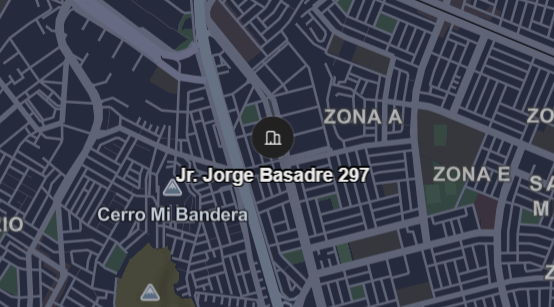
\includegraphics[width=0.55\textwidth]{ubicacion.png}
  \nota{Elaboración propia a partir de Google Maps (2026).}
\end{figure}

\section{Misión, Visión, Objetivo y Valores de la Empresa}

\subsection{Misión}
Diseñar, desarrollar e implementar soluciones informáticas confiables, seguras y adaptadas a las necesidades específicas de las municipalidades peruanas, contribuyendo a la modernización de su gestión administrativa y a la mejora continua de la atención al ciudadano, mediante un servicio técnico cercano y comprometido con cada entidad cliente.

\subsection{Visión}
Consolidarnos, para el año 2030, como la empresa referente a nivel nacional en la estandarización y modernización de los sistemas de gestión municipal, reconocida por la calidad, escalabilidad y sostenibilidad de sus soluciones tecnológicas, y por su aporte a la reducción de la brecha digital entre los gobiernos locales del Perú.

\subsection{Objetivo}
Normalizar progresivamente los sistemas informáticos utilizados por las municipalidades del Perú, reemplazando los desarrollos particularizados y dependientes de infraestructura física o de una sola persona por soluciones web estandarizadas, escalables y de fácil mantenimiento, que optimicen los procesos de gestión municipal y faciliten el acceso a la información para la toma de decisiones.

\subsection{Valores de la Empresa}

\begin{itemize}[leftmargin=1.25cm,itemsep=0pt,topsep=0pt]
  \item \textbf{Compromiso:} con la calidad del servicio brindado a cada municipalidad cliente y con el cumplimiento de los plazos y requerimientos acordados.
  \item \textbf{Confiabilidad:} garantizando la seguridad, disponibilidad e integridad de la información gestionada por los sistemas desarrollados.
  \item \textbf{Innovación:} incorporando de manera constante nuevas tecnologías (como la inteligencia artificial) que aporten valor a la gestión pública local.
  \item \textbf{Responsabilidad social:} entendiendo que las soluciones desarrolladas impactan directamente en la calidad del servicio que las municipalidades ofrecen a los ciudadanos.
  \item \textbf{Adaptabilidad:} ajustando las soluciones tecnológicas a la realidad, presupuesto y capacidad operativa de cada municipalidad atendida.
\end{itemize}

\section{Producto, Mercado y Cliente}

\subsection{Producto}
Consultoría Informática ofrece un sistema integral de gestión municipal orientado al área de rentas y trámites documentarios, que permite automatizar procesos como el registro de contribuyentes y propietarios, la administración del catastro urbano, el procesamiento de transferencias y bajas de propiedades, y la generación de reportes para la toma de decisiones. El producto se entrega actualmente como software de escritorio, aunque se encuentra en proceso de migración hacia una arquitectura web que permita un acceso más flexible y una mejor experiencia de uso para el personal municipal.

\subsection{Mercado}
El mercado objetivo de la empresa está conformado por el sector público local a nivel nacional, específicamente por las municipalidades distritales y provinciales del Perú que requieren digitalizar o modernizar su gestión administrativa. Dado que, según cifras del RENAMU, una parte significativa de los gobiernos locales del país aún no cuenta con sistemas digitales adecuados para sus procesos, este segmento representa un mercado con demanda potencial de crecimiento sostenido, especialmente en municipios distritales de mediana y pequeña escala.

\subsection{Cliente}
Los clientes de Consultoría Informática son las municipalidades peruanas, principalmente aquellas de escala distrital, que requieren soluciones tecnológicas adaptadas a sus procesos internos de gestión de rentas, catastro y trámites documentarios. Entre estos clientes se encuentra actualmente la Municipalidad de San Bartolo, entidad para la cual se desarrolla el presente proyecto de innovación.

\section{Organigrama de la Empresa}

\begin{figure}[H]
  \centering
  \caption{Organigrama de la Empresa}
  \label{fig:organigrama}
  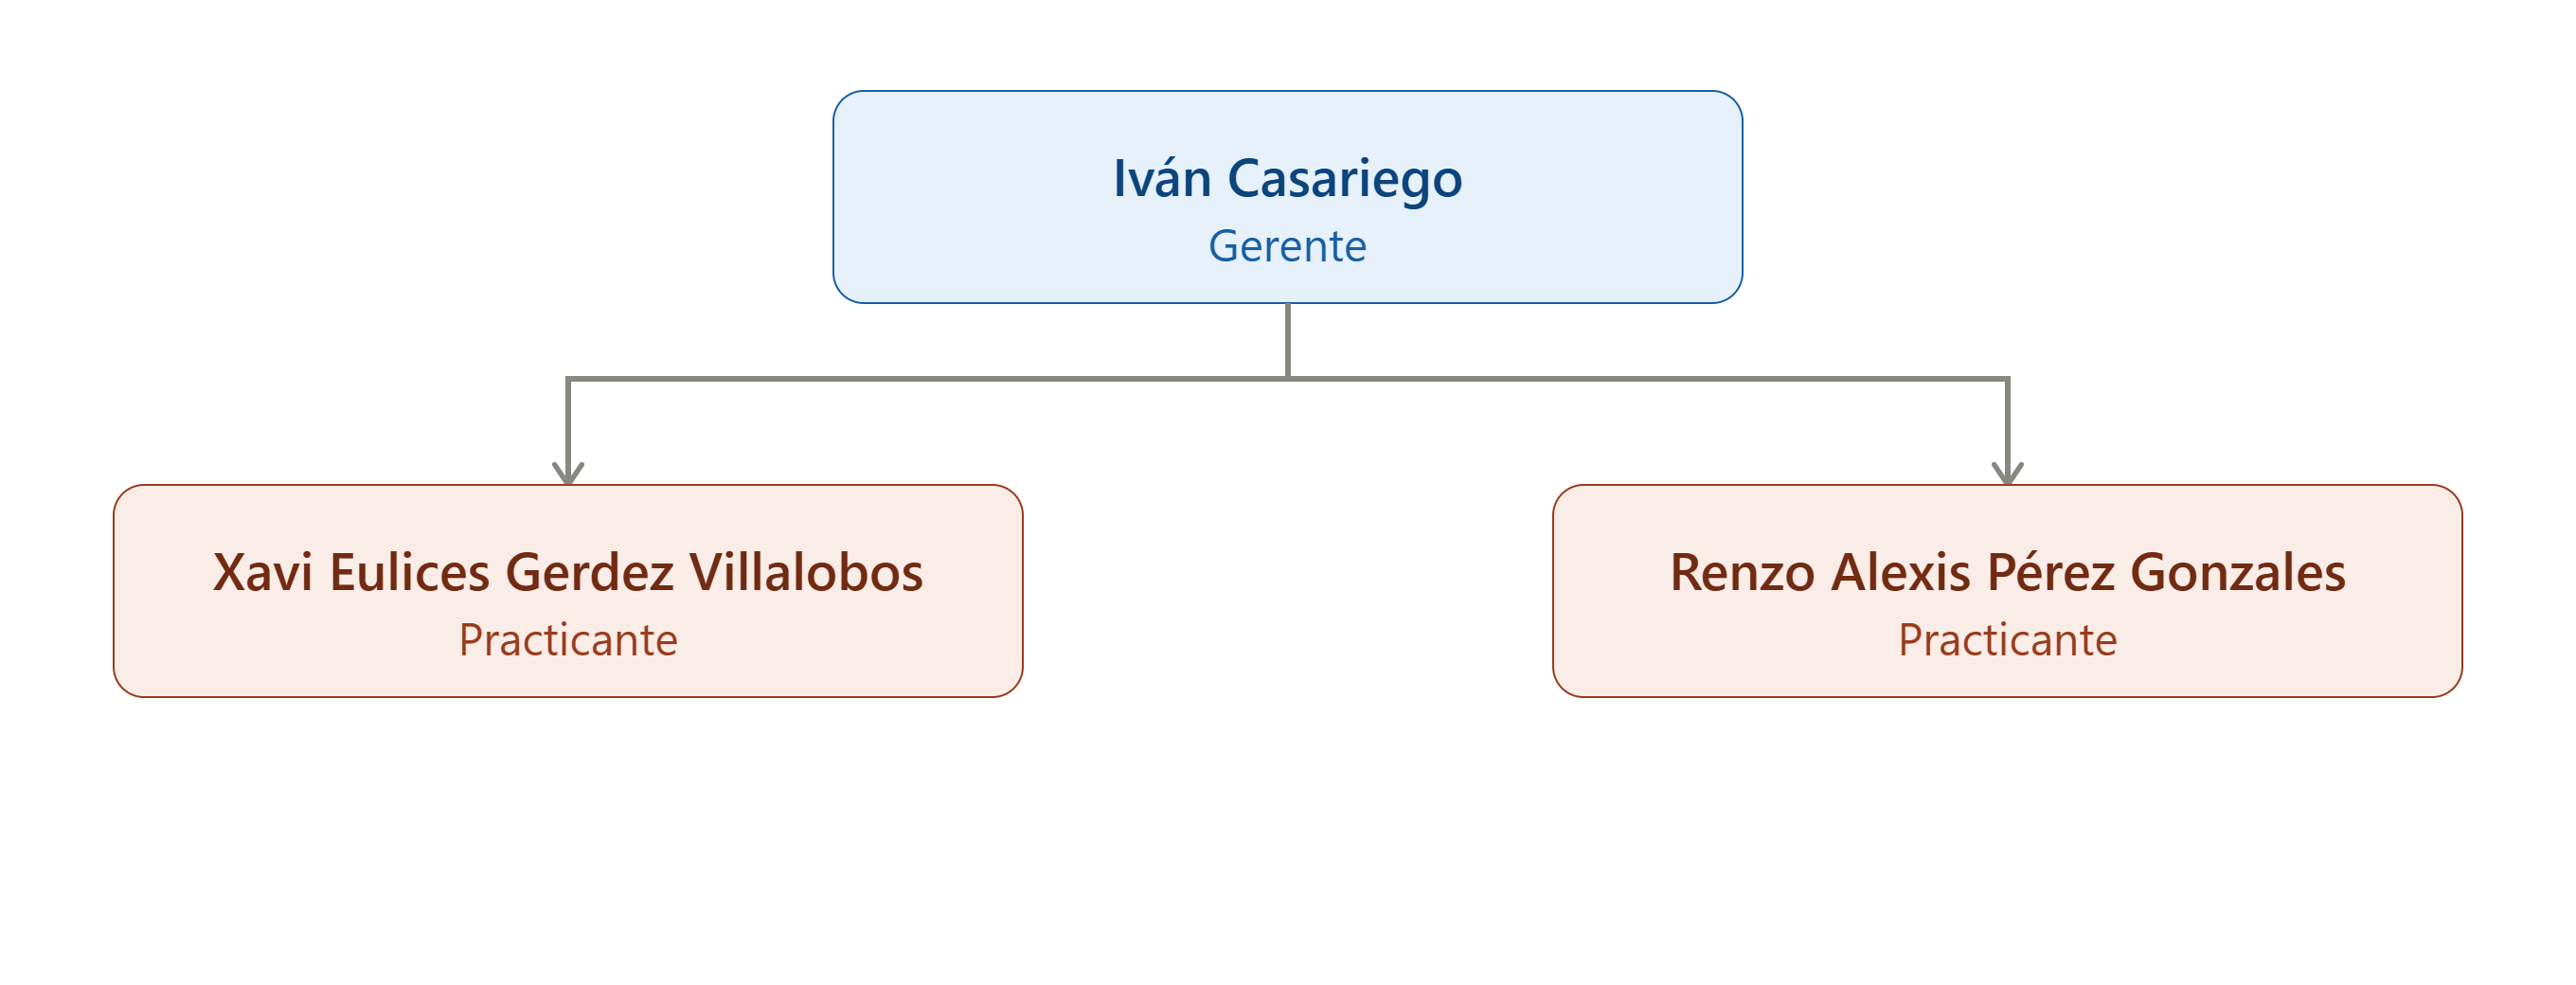
\includegraphics[width=0.9\textwidth]{organigrama.png}
  \nota{Elaboración propia. Estructura organizacional de Consultoría Informática y sus niveles jerárquicos.}
\end{figure}

\section{Otra información relevante de la Empresa donde se desarrollará el Proyecto}

\subsection{Planificación y Gestión de la Entrevista}
En esta sección se describe la entrevista realizada con el encargado del área de Rentas de la Municipalidad de San Bartolo y con el responsable de la empresa, con el fin de identificar la problemática principal junto con sus causas y los beneficios que se obtendrán con la implementación del sistema web, a partir de una lista de preguntas.

\noindent\textbf{Fecha y hora:} \pend{dd/mm/2026 -- hh:mm} \textbf{--- Encargado:} \pend{nombre y cargo del entrevistado}

\noindent\textbf{1. ¿Defina usted sus funciones en la empresa o en el área de Rentas?}\\
\pend{transcribir la respuesta del entrevistado}

\noindent\textbf{2. ¿Por qué desea migrar el sistema actual (Sispredios) a un sistema web?}\\
\pend{transcribir la respuesta del entrevistado}

\noindent\textbf{3. ¿Qué espera obtener a partir de la implementación del sistema web?}\\
\pend{transcribir la respuesta del entrevistado}

\noindent\textbf{4. ¿Cuánto tiempo toma actualmente atender una incidencia o una corrección del sistema?}\\
\pend{transcribir la respuesta del entrevistado}

\noindent\textbf{5. ¿Cómo se decide a qué contribuyentes se envían las cartas de aviso o los valores de cobranza?}\\
\pend{transcribir la respuesta del entrevistado}

\subsection{Contexto del Proyecto: Municipalidad de San Bartolo}
El presente proyecto se desarrolla para la Municipalidad de San Bartolo, cliente de Consultoría Informática, que utiliza Sispredios para administrar el registro de contribuyentes y predios, la emisión de deudas del impuesto predial y los arbitrios, la caja y la cobranza ordinaria y coactiva. El sistema funciona instalado en los equipos de la municipalidad y depende de un servidor físico local, situación que se ha vuelto crítica con el proceso de reubicación del local municipal, ya que cualquier traslado del servidor interrumpe el acceso a la información.

En este contexto, la empresa decidió migrar Sispredios a una plataforma web estandarizada que pueda reutilizarse con otras municipalidades. La primera versión de la nueva base de datos agrupa la información en ocho dominios (administración, contribuyentes, catastro y predios, vehicular, parámetros tributarios, deuda y caja, cobranza y coactivo, y licencias) y, sobre el historial de deudas y pagos registrado durante años, se incorporará un modelo de Machine Learning para estimar el riesgo de morosidad. Como avance, se desarrolló el módulo de Accesibilidad del nuevo sistema (Anexo~\ref{anx:accesibilidad}).

% =====================================================================
% CAPÍTULO II: PLAN DE PROYECTO DE INNOVACIÓN / MEJORA / CREATIVIDAD
% =====================================================================
\chapter{Plan de Proyecto de Innovación / Mejora / Creatividad}

\section{Identificación del Problema Técnico en la Empresa}

\subsection{Problema Local de la Empresa}

Consultoría Informática desarrolla y vende software de gestión a municipalidades, y uno de sus productos es Sispredios, un sistema de gestión tributaria predial desarrollado en Visual FoxPro 9 como aplicación de escritorio. Se trata de un sistema de gran tamaño: el análisis de sus archivos muestra 219 formularios, 202 reportes y 252 tablas en su base de datos principal, que ocupa cerca de 3,5 GB, con alrededor de 1,9 millones de registros en su tabla de cuenta corriente y más de un millón de registros de pagos. % VERIFICAR el significado de la tabla de cuenta corriente al leer el código

Esta tecnología, además, ya no cuenta con respaldo del fabricante: Microsoft mantuvo el soporte extendido de Visual FoxPro hasta enero de 2015 \parencite{taft2007}. A esto se suma que el sistema funciona instalado en equipos locales, por lo que su uso queda limitado a la infraestructura física de cada entidad, y que cada municipalidad atendida cuenta con una solución distinta, construida de manera particular.

El problema principal identificado en la empresa es la \textit{falta de estandarización y sostenibilidad en el desarrollo y soporte de los sistemas de software entregados a las municipalidades}. Para priorizar sus causas se aplicó el método de Pareto (sección~\ref{sec:pareto}). Este problema se origina en las siguientes cuatro causas:

\causa{a}{Falta de estandarización en los sistemas desarrollados}Cada municipalidad atendida cuenta con una solución distinta, lo que dificulta el mantenimiento, la escalabilidad y la reutilización de código entre proyectos.

\causa{b}{Interfaces de usuario poco intuitivas, con un diseño UI/UX obsoleto e incómodo}Es un rasgo propio de las aplicaciones de escritorio antiguas, y dificulta el uso cotidiano del personal municipal.

\causa{c}{Demoras en la atención de soporte técnico}El conocimiento y la carga de trabajo se concentran en una sola persona y no existen procesos ni personal dedicado exclusivamente a las incidencias, situación que se agrava al depender de una tecnología sin soporte oficial.

\causa{d}{Limitación en el acceso a información estadística}Los sistemas actuales no facilitan la generación ni la consulta de reportes consolidados, y el historial de pagos y deudas acumulado durante años no se aprovecha para anticipar la morosidad ni para priorizar la cobranza, por lo que la gestión de cobro se vuelve reactiva. % VERIFICAR con el encargado de la empresa

Esta situación se refleja en la propia instalación de Sispredios. Algunos de sus programas auxiliares conservan rutas fijas a carpetas de otras municipalidades atendidas por la empresa, lo que muestra que el mismo código se copia y se adapta para cada cliente. Además, en la carpeta del sistema se conservan 35 versiones compiladas del ejecutable entre 2020 y 2025, siete de ellas generadas en solo tres días de mayo de 2023, porque cada corrección exige recompilar e instalar de nuevo todo el programa. Por último, para decidir a quién cobrar, el personal trabaja con listados exportados manualmente a hojas de cálculo, de los que se encontraron 20 archivos en la carpeta del sistema. Estos datos se detallan en el análisis cuantitativo del Capítulo~3.

\subsection{Problema Nacional}

A nivel nacional, la falta de modernización de los sistemas informáticos en las municipalidades del Perú constituye un problema estructural que trasciende a una sola entidad o región. \textcite{francoulco2026} menciona que, según datos del Registro Nacional de Municipalidades (RENAMU) del año 2023, del total de 1,891 municipalidades del país, solo el 47,8\,\% cuenta con Mesa de Partes Virtual, mientras que el 52,2\,\% restante aún no ha implementado este tipo de plataformas digitales. Asimismo, el autor señala que mientras el 86,7\,\% de las municipalidades provinciales ya ha implementado sistemas de este tipo, en el ámbito distrital la adopción se reduce al 43,3\,\% \parencite{francoulco2026}.

Esta brecha se refleja en la gestión tributaria. \textcite{romerocarazas2021} advierten una aparente pasividad fiscal en los gobiernos locales del Perú, que prefieren depender de las transferencias del gobierno central antes que desarrollar nuevas estrategias de recaudación, mientras que \textcite{rojasbarbaran2021} realizaron una revisión sistemática sobre la gestión de la recaudación tributaria en las municipalidades del país. En el caso del impuesto predial, \textcite{riosvelasquez2022} reportan que en la Municipalidad Distrital de El Porvenir (Trujillo) la morosidad de este impuesto era de 72\,\% en 2019 y de 79\,\% en 2020, y que bajó a 65\,\% en 2021 tras aplicar beneficios tributarios en forma de descuentos sobre la deuda.

La falta de herramientas tecnológicas aparece también como un factor del problema. \textcite{soriadiaz2022} describen que en la Municipalidad Distrital de Punchana los contribuyentes deben acudir personalmente a realizar sus trámites porque la entidad no cuenta con servicios en línea y su portal web está desactualizado, y señalan que la ausencia de datos actualizados de los contribuyentes limita el aumento de la recaudación.

En conjunto, estos estudios indican que el problema identificado en Consultoría Informática no es un caso aislado: la desigual capacidad tecnológica de los gobiernos locales y las dificultades de cobranza del impuesto predial son problemas nacionales, lo que abre una oportunidad para que soluciones informáticas estandarizadas, con apoyo de analítica de datos, contribuyan a mejorar la gestión municipal.

Además, la recaudación del impuesto predial en el país es sensible a las condiciones económicas de la población. \textcite{cayatopa2026} analizaron la recaudación predial en el Perú entre 2012 y 2023 mediante un modelo de vectores autorregresivos con datos de panel, y encontraron que la pobreza tiene un efecto inverso sobre la recaudación, de $-0{,}21$ antes de la pandemia, que se intensificó a $-0{,}30$ durante y después de ella. Los autores proponen acciones focalizadas para mejorar la recaudación municipal, lo que refuerza la necesidad de herramientas que permitan identificar a qué contribuyentes dirigir primero la gestión de cobranza.

\subsection{Problema Internacional}

A nivel internacional, la falta de digitalización y estandarización en la gestión de trámites municipales es una problemática que afecta de manera generalizada a la región latinoamericana, no siendo exclusiva del Perú. \textcite{bid2018} señalan que, en promedio, un ciudadano latinoamericano necesita 5,4 horas para completar una gestión ante una entidad pública, y que el 25\,\% de los trámites requiere tres interacciones o más con la entidad para resolverse, lo cual evidencia la persistencia de procesos burocráticos lentos y poco eficientes en gran parte de los gobiernos de la región.

Asimismo, el organismo señala que el 29\,\% de los ciudadanos de América Latina reportó haber pagado un soborno en el contexto de un servicio público en el último año \parencite{bid2018}, lo que refleja que la ausencia de sistemas digitales estandarizados no solo genera ineficiencia operativa, sino que también favorece espacios de informalidad y corrupción dentro de la administración pública local.

Esta situación confirma que el problema de fondo ---sistemas de gestión municipal poco estandarizados, dependientes de procesos manuales o de soluciones tecnológicas aisladas--- es una tendencia regional presente en distintos países de Latinoamérica, lo que refuerza la pertinencia de que empresas como Consultoría Informática desarrollen soluciones de software que contribuyan a modernizar y homogeneizar la gestión de los gobiernos locales, no solo en el contexto peruano sino como parte de un desafío compartido a nivel latinoamericano.

\subsection{Formulación del Problema}

\subtitulo{Problema General}

¿De qué manera la implementación de un sistema web de gestión tributaria predial, con un modelo de Machine Learning para estimar el riesgo de morosidad, mejorará la estandarización, el soporte y la sostenibilidad de los sistemas de software que Consultoría Informática brinda a las municipalidades?

\subtitulo{Problemas Específicos}

¿De qué manera la implementación de un sistema web con una arquitectura común y reutilizable (NestJS, React y PostgreSQL) mejorará la estandarización de los sistemas entregados a las municipalidades?

¿De qué manera el diseño de una interfaz web moderna, intuitiva y consistente (React y Tailwind CSS) mejorará la experiencia de uso del personal municipal frente a las interfaces obsoletas de escritorio?

¿De qué manera un sistema web con una única base de código, desplegada y actualizada de forma centralizada, reducirá las demoras en la atención de soporte técnico?

¿De qué manera un modelo de Machine Learning que estime el riesgo de morosidad de los contribuyentes mejorará el acceso a información estadística y la priorización de la cobranza en las municipalidades?

\section{Objetivo del Proyecto de Innovación}

\subsection{Objetivo General}

Implementar un sistema web de gestión tributaria predial, con un modelo de Machine Learning para estimar el riesgo de morosidad, que mejore la estandarización, el soporte y la sostenibilidad de los sistemas de software que Consultoría Informática brinda a las municipalidades.

\subsection{Objetivo Específico}

Desarrollar el sistema web sobre una arquitectura común y reutilizable (NestJS, React y PostgreSQL) para mejorar la estandarización de los sistemas entregados a las municipalidades.

Diseñar una interfaz web moderna, intuitiva y consistente (React y Tailwind CSS) para mejorar la experiencia de uso del personal municipal frente a las interfaces obsoletas de escritorio.

Centralizar el despliegue y la actualización del sistema en una única base de código para reducir las demoras en la atención de soporte técnico.

Entrenar e integrar un modelo de Machine Learning que estime el riesgo de morosidad de los contribuyentes para mejorar el acceso a información estadística y la priorización de la cobranza en las municipalidades.

\section{Antecedentes del Proyecto de Innovación / Mejora / Creatividad (Investigaciones Realizadas)}
\label{sec:antec}

Se revisaron quince investigaciones: cinco antecedentes nacionales, cinco internacionales y cinco artículos científicos. Todas se relacionan con alguno de los dos ejes del proyecto: la gestión tributaria municipal apoyada en sistemas web, y la predicción de la morosidad o del incumplimiento tributario mediante técnicas de Machine Learning. En el Anexo~\ref{anx:antecedentes} se presenta un cuadro resumen.

\subtitulo{Antecedentes Nacionales}

En la tesis para optar el título de Ingeniero en Informática y Sistemas en la Universidad Nacional Agraria de la Selva, sustentada por \textcite{juncoaranciaga2023}, se presenta como título de investigación ``Evaluación comparativa en el desempeño de modelos de machine learning en la predicción de pagadores del impuesto predial de la ciudad de Tingo María para el año 2019''. El problema que aborda es la dificultad de la municipalidad para anticipar qué contribuyentes cumplirán con el pago del impuesto predial, lo que limita la planificación de la cobranza. Para ello, el autor aplicó una encuesta telefónica a 372 contribuyentes sobre factores socioeconómicos y de percepción, evaluó con la prueba Chi cuadrado la influencia de dichos factores en la clasificación de cada contribuyente como ``No pagador'', ``Impuntual'' o ``Pagador'', y entrenó modelos de árbol de decisión, máquinas de vectores de soporte (SVM), vecinos más cercanos (KNN), Naive Bayes, modelos de conjunto y redes neuronales, con validación cruzada de 10 pliegues y optimización de hiperparámetros. Como resultado, los modelos KNN y de redes neuronales obtuvieron las mayores exactitudes, de 97,04\,\% y 96,89\,\% respectivamente, y la prueba de Friedman mostró que las diferencias entre algoritmos eran estadísticamente significativas. Este antecedente es el más cercano al presente proyecto, pues demuestra en una municipalidad peruana que el aprendizaje automático puede clasificar a los contribuyentes según su comportamiento de pago del impuesto predial; a diferencia de dicho estudio, el presente proyecto propone utilizar el historial de deudas y pagos registrado en el propio sistema, en lugar de una encuesta.

En la tesis para optar el título profesional de Ingeniero de Sistemas e Informática en la Universidad Nacional de la Amazonía Peruana, sustentada por \textcite{pacaya2022}, se presenta como título de investigación ``Sistema informático web para la gestión de cobranza en el CETIC de la Municipalidad Distrital de Punchana, año 2021''. El estudio parte de la necesidad de mejorar la gestión de cobranza en dicha dependencia municipal. El objetivo fue desarrollar e implementar un sistema informático web que optimizara esa gestión. Los autores aplicaron un enfoque cuantitativo de nivel tecnológico aplicado, con diseño preexperimental, transversal y prospectivo, y midieron los tiempos de operación con cronómetro en 20 registros de pagos, 20 de matrículas, 10 de personal nuevo y 10 de generación de reportes. Como resultado, reportaron una efectividad de 126\,\% en el registro de pagos, 114\,\% en el registro de matrículas, 136\,\% en el registro de personal y 15,246\,\% en la generación de reportes de gestión, cifra muy superior a las demás, que los autores reportan tal como la obtuvieron. Se concluye que la implementación del sistema web optimiza la gestión de cobranza, por lo que se acepta la hipótesis de investigación. Este antecedente respalda la propuesta de reemplazar procesos de cobranza poco automatizados por un sistema web, y su forma de medir el efecto mediante tiempos de operación es aplicable al presente proyecto.

En la tesis de grado de la Universidad Nacional de la Amazonía Peruana, sustentada por \textcite{laulate2025}, se presenta como título de investigación ``Sistema web para la gestión de rentas de la Municipalidad Provincial de Maynas-2024''. El problema que aborda es la baja eficiencia operativa de la gestión de rentas municipales en tres procesos: la consulta de deudas, los pagos en línea y la entrega de notificaciones. El objetivo fue optimizar dicha eficiencia mediante un sistema web que además mejorara la experiencia de usuario. La metodología fue preexperimental con enfoque cuantitativo: se analizaron datos de 30 contribuyentes antes y después de implementar el sistema, con encuestas de usabilidad SUS y formularios de observación para medir los tiempos de proceso. Como resultados, el tiempo de consulta de deudas bajó de 16,47 a 2,50 minutos, el de pago de deudas de 18,43 a 2,50 minutos y el de entrega de notificaciones de 26,67 a 2,00 minutos, y el puntaje SUS promedio fue de 51,75, que indica una usabilidad moderada. Los autores concluyen que el sistema reduce los tiempos y estandariza los procesos, y recomiendan actualizarlo periódicamente, capacitar a los usuarios e incorporar recordatorios automáticos y más opciones de pago. Este antecedente muestra, en una municipalidad peruana, el efecto de un sistema web sobre la gestión de rentas, y su recomendación de incorporar recordatorios automáticos se vincula con la priorización de la cobranza que persigue el presente proyecto.

En la tesis para optar el título profesional de Contador Público en la Universidad Peruana Unión, sustentada por \textcite{campos2024}, se presenta como título de investigación ``La morosidad como predictor de la recaudación del impuesto predial de la Municipalidad Provincial de San Marcos -- Cajamarca''. La problemática es la baja recaudación del impuesto predial en dicha municipalidad, vinculada al pago tardío de los contribuyentes. El objetivo fue determinar la influencia de los factores de la morosidad en la recaudación del impuesto predial. Se aplicó un enfoque cuantitativo, con diseño descriptivo no experimental y una muestra no probabilística por conveniencia de 250 pobladores mayores de 18 años, a quienes se encuestó mediante formularios en línea; el análisis se realizó con el coeficiente alfa de Cronbach, la prueba de Kolmogorov-Smirnov y la correlación de Spearman en SPSS. Como resultados, la correlación global entre morosidad y recaudación fue de 0,578 (moderada y positiva), y por factores fue de 0,335 para el actitudinal, 0,401 para el social, 0,551 para el económico y 0,549 para el institucional. Se concluye que los factores actitudinales, sociales, económicos e institucionales contribuyen a la falta de pago. Este antecedente identifica factores que explican la morosidad predial, que el presente proyecto busca capturar de manera objetiva a partir del historial de pagos y no de encuestas.

En la tesis de Maestría en Gestión Pública presentada en la Universidad César Vallejo, sustentada por \textcite{paredes2022}, se presenta como título de investigación ``Cultura tributaria y su incidencia en la morosidad del impuesto predial en la Municipalidad Distrital de San Martín de Porres''. La problemática es la alta morosidad del impuesto predial en el distrito, de 44,63\,\% en 2019 y 55,12\,\% en 2020, lo que dificulta el cumplimiento de las metas de recaudación. El objetivo fue determinar cómo la cultura tributaria afecta la morosidad. La investigación fue básica, cuantitativa y correlacional-causal, con diseño no experimental y transversal; se encuestó a 100 contribuyentes mediante muestreo intencional y los datos se analizaron con regresión logística en SPSS. Como resultados, la cultura tributaria afecta significativamente la morosidad, con un R$^2$ de Nagelkerke de 0,22; la dimensión del sistema tributario fue significativa (10,9\,\%), al igual que el cumplimiento fiscal (6,5\,\%), mientras que la conciencia tributaria no lo fue. Se concluye que la cultura tributaria explica cerca del 22\,\% de la variación de la morosidad. Este antecedente sugiere que una parte importante de la morosidad no se explica solo por actitudes de los contribuyentes, por lo que otras fuentes de información, como su historial de pagos, pueden aportar a su estimación.

\subtitulo{Antecedentes Internacionales}

En la tesis de Maestría en Ciencias de la Computación y Comercio Electrónico de la Escuela Politécnica Nacional del Ecuador, sustentada por \textcite{ordonez2020}, se presenta como título de investigación ``Modelo para predecir las deudas de los contribuyentes con alta probabilidad de no pago en la administración tributaria''. El problema planteado es que las administraciones tributarias cuentan con personal, herramientas y tiempo limitados, por lo que necesitan recuperar las deudas en una etapa temprana, cuando la cobranza resulta menos costosa, e identificar cuáles tienen mayor probabilidad de no ser pagadas. El objetivo fue construir, mediante un proceso de minería de datos, un modelo que prediga las deudas con alta probabilidad de no pago para apoyar la toma de decisiones en la gestión de la deuda. Para ello, el autor aplicó análisis de supervivencia con técnicas de aprendizaje automático sobre un conjunto de deudas de una administración tributaria. Como resultado, identificó tres grupos de deudores con comportamientos de pago similares y obtuvo un desempeño de hasta 90\,\% medido con el índice de concordancia al estimar el tiempo de pago de los contribuyentes. Este trabajo respalda el enfoque del presente proyecto de estimar el riesgo a nivel de cada deuda para priorizar la cobranza con recursos limitados.

En la tesis para optar el título de Ingeniera Civil Industrial en la Universidad de Chile, sustentada por \textcite{cifuentes2016}, se presenta como título de investigación ``Modelo predictivo del no pago de giros relacionados con el Formulario 29 para el Servicio de Impuestos Internos de Chile''. El problema es que los giros que emite la administración tributaria por pagos incorrectos presentan bajas tasas de pago, lo que reduce la recaudación. El objetivo fue construir un modelo que estime la probabilidad de que un giro no sea pagado, con énfasis en las micro y pequeñas empresas, para priorizar acciones preventivas o correctivas. La autora construyó 50 variables sobre los contribuyentes, sus negocios y sus pagos a partir de las bases de datos de la institución, depuró un conjunto de 292,940 giros, entrenó los modelos con el 60\,\% de los datos y comparó árboles de decisión, incluido Random Forest, con regresión logística; finalmente seleccionó un árbol CHAID por su interpretabilidad. Como resultados, el modelo seleccionado alcanzó una exactitud de 78,2\,\%, una precisión de 83,1\,\% y una especificidad de 65,6\,\%, y las variables más influyentes fueron el tipo de giro, la relación entre el monto del giro y el pago mensual promedio, y el monto de la deuda. Se concluye que los casos con alta probabilidad de no pago deben revisarse en busca de malas prácticas contables, mientras que los de baja probabilidad pueden abordarse con campañas educativas, y se recomienda priorizar la cobranza en los giros con mayor probabilidad de no pago. Este antecedente respalda el uso de variables derivadas de la deuda y el historial de pago, y la preferencia por modelos interpretables para el personal que debe actuar sobre el resultado.

En la tesis de Maestría en Ingeniería -- Analítica de la Universidad Nacional de Colombia, sede Medellín, sustentada por \textcite{orozco2023}, se presenta como título de investigación ``Una propuesta de modelo para la determinación de la probabilidad de recaudo del impuesto vehicular en Antioquia''. El problema es que las administraciones tributarias necesitan herramientas de apoyo a la toma de decisiones, como la priorización de los procesos de fiscalización, y un análisis más profundo de sus datos. El objetivo fue desarrollar un modelo que estime la probabilidad de recaudo del impuesto vehicular en el departamento de Antioquia. Tras una revisión de la literatura sobre modelos de clasificación y regresión, el autor estudió el contexto del negocio y los datos disponibles, y diseñó un modelo que entrega una estimación de probabilidad para cada contribuyente. Como resultado, el modelo Random Forest obtuvo las mejores métricas entre los evaluados, y se concluye que es el que mejor se ajusta a las necesidades del problema. Este antecedente aplica el enfoque propuesto a un impuesto subnacional y entrega una probabilidad por contribuyente, que es la forma de resultado prevista para el presente proyecto.

En la tesis de maestría de la Namibia University of Science and Technology, sustentada por \textcite{sifani2025}, se presenta como título de investigación ``Predictive Modelling of Taxpayer Compliance Behaviour Using Machine Learning at NamRA'' (Modelado predictivo del comportamiento de cumplimiento tributario mediante Machine Learning en la Namibia Revenue Agency). El objetivo fue explorar el uso del aprendizaje automático para predecir el comportamiento de cumplimiento de los contribuyentes de dicha agencia. Se ajustaron varios algoritmos de clasificación mediante validación cruzada de cinco pliegues, con búsqueda en cuadrícula y búsqueda aleatoria de hiperparámetros en scikit-learn, y se usaron las técnicas SHAP y LIME para interpretar los resultados. Como resultados, la exactitud validada de los modelos estuvo entre 64\,\% y 68\,\%, y el mejor fue Random Forest optimizado con 68\,\%; los factores más influyentes fueron el grupo de ingreso, el periodo de la pandemia de COVID-19, la oficina de registro y el estado civil. Se concluye que el ajuste de hiperparámetros mejoró el desempeño y que el aprendizaje automático puede apoyar la gestión del cumplimiento basada en datos, aunque el autor reconoce que la exactitud es modesta y recomienda, como trabajo futuro, usar datos más ricos y evaluar la equidad. Este antecedente advierte que los modelos de este tipo deben usarse como apoyo a la decisión y no como decisión automática, criterio que adopta el presente proyecto.

En la tesis para optar el título de Ingeniero en Informática de la Escuela Superior Politécnica Agropecuaria de Manabí, Ecuador, sustentada por \textcite{pinargote2018}, se presenta como título de investigación ``Aplicación Web de consultas en línea de valores prediales en el Gobierno Autónomo Descentralizado Municipal del Cantón Junín''. El problema es que las consultas de valores prediales se atendían de forma manual en las áreas de Recaudación y de Tecnologías de la Información, lo que recargaba al personal y a los ciudadanos. El objetivo fue desarrollar una aplicación web que permitiera realizar esas consultas en línea. La autora aplicó razonamiento inductivo-deductivo para estudiar los procesos existentes, desarrolló la aplicación por fases con la metodología MIDAS, recogió datos mediante observación de campo y entrevistas, y empleó PHP y SQL, entre otras herramientas. Como resultado, obtuvo una aplicación que sistematiza los procesos de consulta de valores prediales y cuyo funcionamiento verificó mediante pruebas. Se concluye que la aplicación ayudó considerablemente a los empleados municipales y a los usuarios. Este antecedente respalda la viabilidad de llevar procesos prediales municipales a una aplicación web.

\subtitulo{Artículos Científicos}

En el artículo de investigación publicado por \textcite{leekim2024}, titulado ``Deep Learning-based Delinquent Taxpayer Prediction: A Scientific Administrative Approach'', los autores señalan que, aunque la predicción del riesgo crediticio ha sido ampliamente estudiada, su aplicación a la predicción de la morosidad tributaria se encuentra poco explorada. Proponen predecir la morosidad de los impuestos locales de contribuyentes individuales en la República de Corea, combinando información crediticia (historial de préstamos, registros de morosidad y uso de tarjetas de crédito) con información tributaria pública. Para ello compararon modelos de aprendizaje automático y de aprendizaje profundo, entre ellos redes neuronales convolucionales (CNN), redes de memoria a corto y largo plazo (LSTM) y modelos secuencia a secuencia (seq2seq), y concluyeron que el modelo CNN obtuvo la mejor capacidad predictiva. Los autores destacan que una mejor predicción de la morosidad permite a las administraciones tributarias asignar sus recursos administrativos de forma más eficiente, objetivo que coincide con la priorización de la cobranza que persigue el presente proyecto.

En el artículo publicado por \textcite{ippolito2020}, titulado ``Tax Crime Prediction with Machine Learning: A Case Study in the Municipality of São Paulo'', los autores utilizaron las bases de datos de la propia municipalidad de São Paulo para predecir delitos contra el impuesto municipal sobre servicios. Su metodología comprendió la selección de variables, la extracción y partición de los datos, el entrenamiento y prueba de modelos, y su evaluación y validación. Como resultado, el algoritmo Random Forest obtuvo el mejor desempeño frente a otros algoritmos de aprendizaje automático y mostró buena capacidad de generalización con datos nuevos, lo que permitió orientar mejor los planes de fiscalización de la municipalidad. Este caso demuestra que los datos que un gobierno local ya almacena en sus sistemas son suficientes para construir modelos predictivos útiles para la gestión tributaria.

En el artículo publicado por \textcite{ourdani2024} en el \textit{IAES International Journal of Artificial Intelligence}, titulado ``Towards a new approach to maximize tax collection using machine learning algorithms'' (Hacia un nuevo enfoque para maximizar la recaudación tributaria mediante algoritmos de Machine Learning), los autores señalan que cobrar de manera eficiente las deudas tributarias es un desafío para las autoridades tributarias locales de Marruecos. El objetivo fue examinar cómo el aprendizaje automático y nuevas estrategias pueden hacer más eficiente esa cobranza. La metodología consistió en segmentar a los contribuyentes, a partir de un gran conjunto de datos de su comportamiento de pago, según su probabilidad de incumplimiento o de acumular deuda, lo que permite identificar a los deudores de alto riesgo, y en proponer estrategias basadas en economía conductual para intervenciones más dirigidas. Como resultado, los autores reportan que la segmentación es efectiva y que casos reales de cobranza de deuda tributaria local muestran el impacto de las estrategias, aunque el resumen no presenta cifras. Se concluye que los métodos basados en datos ayudan a las autoridades locales a mejorar su eficiencia y sus ingresos, pues identificar con exactitud a los deudores de alto riesgo y aplicar acciones adaptadas permite aumentar la recaudación y reducir los recursos desperdiciados.

En la ponencia presentada por \textcite{benedetto2026} en el Simposio Doctoral del 29.º Congreso Iberoamericano de Ingeniería de Software, titulada ``Modelos de Inteligencia Artificial Aplicados a la Gestión de la Mora en las Administraciones Tributarias Subnacionales'', el autor señala que la morosidad afecta la sostenibilidad fiscal, la equidad tributaria y la eficiencia del gasto público, y que los métodos tradicionales de cobranza son reactivos, se basan en reglas estáticas y dependen de procesos manuales. El objetivo es diseñar un modelo basado en Big Data e inteligencia artificial que haga más eficiente la gestión de la morosidad. La propuesta combina algoritmos predictivos que anticipan el incumplimiento, modelos de segmentación automática de contribuyentes por perfil de riesgo y mecanismos de automatización de las estrategias de cobranza, bajo un enfoque de investigación en ciencia del diseño y con datos históricos de recaudación y de comportamiento de pago. Los resultados son preliminares: los modelos predictivos identificarían los patrones de morosidad con mayor precisión que los enfoques tradicionales, aunque el trabajo se encuentra en una etapa intermedia y no reporta métricas. El autor espera que el aporte sea relevante para la investigación y para la práctica de la administración pública. Este antecedente coincide con el problema de la cobranza reactiva identificado en el presente proyecto.

En el artículo publicado por \textcite{debortoli2017} en la \textit{Revista Interdisciplinar de Ciência Aplicada}, titulado ``Proposal for Migration from the Municipal Collection System to the Tax Administration System for Serra Gaúcha City Halls'' (Propuesta de migración del sistema municipal de recaudación al sistema de administración tributaria para las alcaldías de Serra Gaúcha), los autores señalan que varias ciudades del estado de Río Grande do Sul utilizan un sistema tributario desarrollado en COBOL, de unos diez años de antigüedad, que no puede integrarse con aplicaciones web y debe reemplazarse sin interrumpir los servicios a la comunidad. El objetivo es describir una metodología de migración de software que establezca la alineación de las tecnologías de la información con los procesos de las alcaldías, para lo cual se propone un enfoque basado en la guía PMBOK. El resumen del artículo no presenta resultados ni conclusiones, pues describe la metodología propuesta. Este antecedente es cercano al presente proyecto porque aborda la migración de un sistema tributario municipal heredado hacia una plataforma web, como la que se plantea para Sispredios.

\section{Justificación del Proyecto de Innovación / Mejora / Creatividad}

Para elegir los tipos de justificación se analizó cuáles se relacionan directamente con el proyecto. Se consideran la justificación tecnológica, porque el problema nace de una tecnología sin soporte y la solución es una nueva arquitectura de software; la social, porque el sistema lo usan funcionarios municipales y sus resultados llegan a los vecinos; la legal, porque el sistema automatiza procesos regulados por normas tributarias y maneja datos personales; y la económica, porque las causas del problema generan pérdidas que se cuantifican en el Capítulo~3. No se plantea una justificación teórica, porque el proyecto no busca generar conocimiento teórico nuevo sino aplicar técnicas ya validadas, ni una justificación personal.

\subsection{Justificación Tecnológica}

Sispredios fue desarrollado en Visual FoxPro 9, una tecnología cuyo soporte extendido terminó en enero de 2015 \parencite{taft2007}, y funciona como aplicación de escritorio instalada en equipos locales y dependiente de un servidor físico. El proyecto se justifica porque reemplaza esa base por una arquitectura web con tecnologías vigentes y de uso extendido: NestJS y TypeScript en el servidor, React y Tailwind CSS en la interfaz, y PostgreSQL con Prisma como base de datos. Esta arquitectura permite acceder al sistema desde cualquier lugar con conexión a internet, desplegar y actualizar una única versión de forma centralizada, y reutilizar el mismo producto en otras municipalidades en lugar de mantener una copia distinta por cliente.

Además, el sistema incorpora desde su inicio un control de acceso basado en roles y niveles, con autenticación mediante tokens JWT (Anexo~\ref{anx:accesibilidad}), y reserva un componente de Machine Learning que aprovechará el historial de deudas y pagos acumulado durante años, que hoy no se utiliza para anticipar la morosidad.

\subsection{Justificación Social}

El proyecto beneficia, en primer lugar, al personal de las áreas de Rentas, Caja y Cobranza de la Municipalidad de San Bartolo, que podrá acceder al sistema desde cualquier lugar con conexión a internet, sin depender de un servidor físico ni de los equipos donde se instaló la aplicación de escritorio, y con una interfaz web más clara que reduce la curva de aprendizaje. En segundo lugar, beneficia a los vecinos del distrito, porque una atención más ágil en ventanilla y una cobranza ordenada se traducen en un mejor servicio y en información más confiable sobre sus deudas. Además, el modelo de riesgo de morosidad permite que la municipalidad oriente primero sus recordatorios y facilidades de pago hacia los contribuyentes con mayor probabilidad de atrasarse, antes de que su deuda pase a cobranza coactiva, etapa en la que se generan costas, embargos y mayor carga para el vecino. Finalmente, al mejorar la recaudación del impuesto predial, la municipalidad dispone de más recursos para financiar los servicios públicos locales que recibe la comunidad.

\subsection{Justificación Legal}

El proyecto se sustenta en el Decreto Legislativo N.\textsuperscript{o}~1412, Ley de Gobierno Digital \parencite{dleg1412}, que establece el marco para el uso de las tecnologías digitales en las entidades de la administración pública, entre ellas los gobiernos locales, con el fin de mejorar la prestación de servicios a los ciudadanos. Asimismo, la Ley N.\textsuperscript{o}~31814 \parencite{ley31814} promueve el uso de la inteligencia artificial en favor del desarrollo económico y social del país, en un entorno seguro, ético y responsable, lo que respalda la incorporación del modelo de Machine Learning dentro del sistema.

En cuanto al dominio tributario, el sistema automatiza procesos regulados por el Texto Único Ordenado de la Ley de Tributación Municipal \parencite{tuoltm}, que define el impuesto predial y su forma de cálculo, y por el Texto Único Ordenado del Código Tributario \parencite{codigotributario}, que regula, entre otros aspectos, los intereses moratorios y el procedimiento de cobranza. La cobranza coactiva se rige por la Ley de Procedimiento de Ejecución Coactiva \parencite{ley26979}. Por último, el tratamiento de los datos de los contribuyentes se rige por la Ley N.\textsuperscript{o}~29733, Ley de Protección de Datos Personales \parencite{ley29733}; por ello, el modelo de Machine Learning trabajará con identificadores anonimizados, sin utilizar nombres ni documentos de identidad, y su resultado será solo un apoyo para que el personal priorice la cobranza, no una decisión automática.

\subsection{Justificación Económica}
\label{sec:just-econ}

El proyecto se justifica económicamente porque las cuatro causas del problema generan pérdidas que hoy asume la empresa y la municipalidad. Cada actualización del ejecutable consume horas del desarrollador y detiene el trabajo del personal municipal; solo por este concepto, y con valores mínimos referenciales, se estima una pérdida de S/~2,154.60 entre 2020 y 2025 (Tabla~\ref{tab:perdidas}). A ello se suman las horas que se duplican al mantener una versión distinta por municipalidad, el tiempo que el personal pierde con una interfaz obsoleta y el costo de una cobranza que actúa cuando la deuda ya venció, cuya cuantificación detallada se presenta en la sección~\ref{sec:perdidas}.

Con un sistema web de una única base de código, cada corrección se despliega una sola vez para todas las municipalidades, por lo que se reducen las horas de mantenimiento y las paradas de trabajo. Además, la experiencia en otras municipalidades indica que una mejor gestión de la cobranza puede elevar la recaudación: \textcite{riosvelasquez2022} reportan que la morosidad del impuesto predial en El Porvenir bajó de 79\,\% en 2020 a 65\,\% en 2021 tras aplicar beneficios tributarios, y \textcite{ourdani2024} concluyen que identificar con exactitud a los deudores de alto riesgo permite aumentar la recaudación y reducir los recursos desperdiciados.

\section{Marco Teórico y Conceptual}
\label{sec:marco}

\subsection{Fundamento teórico del Proyecto de Innovación / Mejora / Creatividad}

Las variables del estudio son dos. La \textbf{variable independiente} es el \textit{sistema web de gestión tributaria predial con Machine Learning}, es decir, la solución que se implementa. La \textbf{variable dependiente} es la \textit{gestión de la cobranza del impuesto predial}, es decir, el proceso que se busca mejorar y sobre el que actúa el sistema. Cada variable se desarrolla a continuación en una jerarquía de temas y subtemas, y cada tema cierra con su relación con el sistema; la Tabla~\ref{tab:jerarquia} (Anexo~\ref{anx:jerarquia}) resume esta jerarquía.

\subsubsection{Variable independiente: Sistema web de gestión tributaria predial con Machine Learning}

La variable independiente se organiza en cuatro temas: el sistema informático, la aplicación web, la seguridad y el control de acceso, y el Machine Learning.

\noindent\textbf{A) Sistema informático.} \textcite{raya2014} definen un sistema informático como un conjunto de partes interrelacionadas que emplea un ordenador con dispositivos programables para capturar, almacenar y procesar datos (p.~18). Los autores precisan que, aunque su estructura puede dividirse en partes, funcionalmente es indivisible, ya que un sistema informático al que le falta alguno de sus componentes deja de funcionar; dichos componentes son el físico (hardware), el lógico (software) y el humano (p.~18).

\noindent\textbf{A.1) Componente físico (hardware).} Es el conjunto de equipos sobre los que se ejecuta el sistema. \textit{Relación con el sistema:} en el proyecto corresponde al servidor donde se despliega la aplicación y a los equipos de los funcionarios, que solo necesitan un navegador; esto elimina la dependencia de un servidor físico instalado en la municipalidad.

\noindent\textbf{A.2) Componente lógico (software).} Comprende el software de base, que permite el funcionamiento del equipo (sistema operativo y gestor de base de datos), y el software de aplicación, que resuelve las tareas del usuario. \textit{Relación con el sistema:} el software de base es PostgreSQL y el entorno de ejecución Node.js; el software de aplicación es el sistema web de rentas, formado por el servidor (NestJS) y la interfaz (React).

\noindent\textbf{A.3) Componente humano.} Son las personas que operan y mantienen el sistema. \textit{Relación con el sistema:} corresponde al personal de Rentas, Caja y Cobranza de la municipalidad, y al equipo de desarrollo y soporte de la empresa.

\noindent\textbf{B) Aplicación web y arquitectura cliente-servidor.} Una aplicación web es un sistema al que se accede mediante un navegador a través de internet, sin necesidad de instalarlo en cada equipo. \textcite{fielding2000} describe en su tesis doctoral el estilo arquitectónico REST (\textit{Representational State Transfer}) para sistemas distribuidos, que se basa en restricciones como la separación entre cliente y servidor, la comunicación sin estado entre solicitudes, la posibilidad de almacenar respuestas en caché, una interfaz uniforme y una organización en capas. \textit{Relación con el sistema:} el servidor del proyecto expone una API que sigue estos principios y que consume la interfaz en React; esta separación permite cambiar la interfaz sin tocar la lógica de negocio y reutilizar el mismo servidor en distintas municipalidades, lo que ataca directamente la causa de falta de estandarización.

\noindent\textbf{C) Seguridad y control de acceso.} Un sistema que administra datos tributarios debe controlar quién ingresa y qué puede hacer.

\noindent\textbf{C.1) Control de acceso basado en roles (RBAC).} \textcite{sandhu1996} presentan una familia de modelos en la que los permisos se asocian a roles y los usuarios se asignan a los roles que les corresponden, lo que simplifica la administración de la seguridad frente a asignar permisos usuario por usuario. \textit{Relación con el sistema:} el módulo de Accesibilidad del proyecto aplica este modelo: cada pantalla y función es un \textit{nivel}, cada \textit{rol} reúne los niveles que necesita y cada \textit{usuario} tiene un rol (Anexo~\ref{anx:accesibilidad}).

\noindent\textbf{C.2) Autenticación con tokens JWT.} El JSON Web Token es, según \textcite{rfc7519}, un medio compacto y seguro para URL de representar información (\textit{claims}) que se transfiere entre dos partes, y que puede firmarse para verificar su integridad. \textit{Relación con el sistema:} al ingresar, el usuario recibe un token que lleva sus niveles; cada servicio del servidor verifica el nivel exigido leyendo el token, sin consultar la base de datos en cada solicitud, y las contraseñas se almacenan cifradas con bcrypt.

\noindent\textbf{D) Machine Learning.} \textcite{mitchell1997} define el aprendizaje automático de la siguiente manera: ``se dice que un programa de computadora aprende de la experiencia E con respecto a una clase de tareas T y una medida de desempeño P, si su desempeño en las tareas de T, medido por P, mejora con la experiencia E'' (p.~2). \textit{Relación con el sistema:} la tarea T es estimar si una deuda tributaria será pagada con atraso o no será pagada; la experiencia E es el historial de deudas y pagos registrado en el sistema; y la medida P son métricas de clasificación como el área bajo la curva y el porcentaje de morosos reales identificados entre los contribuyentes con mayor puntaje de riesgo.

\noindent\textbf{D.1) Aprendizaje supervisado y clasificación.} En el aprendizaje supervisado el algoritmo aprende a partir de ejemplos cuyo resultado ya se conoce; cuando ese resultado es una categoría (por ejemplo, ``pagó a tiempo'' o ``pagó con atraso'') el problema se denomina de clasificación \parencite{mitchell1997}. \textit{Relación con el sistema:} cada deuda histórica con su desenlace de pago es un ejemplo con el que se entrena el modelo de riesgo.

\noindent\textbf{D.2) Modelos de conjunto: Random Forest y Gradient Boosting.} \textcite{breiman2001} define Random Forest como una combinación de árboles de decisión en la que cada árbol depende de los valores de un vector aleatorio muestreado de forma independiente, y la predicción resulta del conjunto de árboles. \textcite{friedman2001} propone el \textit{gradient boosting}, que construye un modelo aditivo de forma progresiva, añadiendo en cada paso un nuevo modelo que corrige los errores del conjunto anterior. \textit{Relación con el sistema:} varios antecedentes obtuvieron su mejor desempeño con Random Forest \parencite{ippolito2020,orozco2023,sifani2025}, por lo que el proyecto lo comparará con gradient boosting y con una regresión logística como referencia.

\noindent\textbf{D.3) Evaluación de modelos de clasificación.} \textcite{fawcett2006} explica que las gráficas ROC permiten visualizar, organizar y seleccionar clasificadores según su desempeño, y que el área bajo la curva (AUC) resume en un solo valor la capacidad del clasificador para distinguir entre las clases. \textit{Relación con el sistema:} el AUC será la métrica principal para elegir el modelo de riesgo de morosidad, complementada con el porcentaje de morosos reales identificados entre los contribuyentes con mayor puntaje.

\subsubsection{Variable dependiente: Gestión de la cobranza del impuesto predial}

La variable dependiente se organiza en cuatro temas: el impuesto predial, la morosidad tributaria, la cobranza ordinaria y coactiva, y la priorización de la cobranza según el riesgo.

\noindent\textbf{A) Impuesto predial.} De acuerdo con el artículo 8 del Texto Único Ordenado de la Ley de Tributación Municipal, el impuesto predial es de periodicidad anual y grava el valor de los predios urbanos y rústicos; su recaudación, administración y fiscalización corresponden a la municipalidad distrital donde se ubica el predio \parencite{tuoltm}. \textit{Relación con el sistema:} es el principal tributo que gestiona el sistema propuesto y la base de la cuenta corriente de cada contribuyente, donde se registra la deuda por tributo, año y cuota.

\noindent\textbf{B) Morosidad tributaria.} La morosidad tributaria se presenta cuando el contribuyente no cumple con pagar su deuda dentro del plazo establecido. Según el artículo 33 del Texto Único Ordenado del Código Tributario, el monto del tributo no pagado dentro de los plazos indicados devenga un interés moratorio \parencite{codigotributario}. Su magnitud puede ser alta: en el distrito de San Martín de Porres, estudiado por \textcite{paredes2022}, la morosidad predial fue de 44,63\,\% en 2019 y 55,12\,\% en 2020. \textit{Relación con el sistema:} el sistema calcula la mora de cada deuda y es la variable que el modelo de Machine Learning busca anticipar.

\noindent\textbf{C) Cobranza ordinaria y coactiva.} Cuando la deuda persiste, la administración emite valores como la orden de pago o la resolución de determinación y, finalmente, puede iniciar el procedimiento de cobranza coactiva, que se rige por la Ley de Procedimiento de Ejecución Coactiva \parencite{ley26979}. \textit{Relación con el sistema:} el sistema registra las cartas de aviso, los valores, los convenios de fraccionamiento y los expedientes coactivos (Tabla~\ref{tab:causa4}); el área de Rentas decide hoy a quién dirigir cada acción sin una estimación previa del riesgo.

\noindent\textbf{D) Priorización de la cobranza según el riesgo.} Las administraciones tributarias cuentan con personal y tiempo limitados, por lo que les conviene actuar primero sobre las deudas con mayor probabilidad de no pago \parencite{ordonez2020}. Los métodos tradicionales de cobranza son reactivos y dependen de procesos manuales \parencite{benedetto2026}, mientras que una mejor predicción de la morosidad permite asignar los recursos administrativos de forma más eficiente \parencite{leekim2024}. \textit{Relación con el sistema:} el puntaje de riesgo que genera el modelo se muestra al personal de Rentas como apoyo para ordenar su trabajo, sin reemplazar su decisión.

\subsection{Marco conceptual}

Los siguientes términos se utilizan a lo largo del documento y corresponden al dominio de la gestión tributaria municipal, a la seguridad del sistema y a la documentación de la base de datos del sistema desarrollado.

\begin{itemize}[leftmargin=1.25cm,itemsep=0pt,topsep=0pt]
  \item \textbf{Predio:} inmueble formado por el terreno y lo construido sobre él; puede ser una casa, un local, un terreno vacío o una cochera.
  \item \textbf{Autovalúo:} valor oficial del predio en soles, calculado cada año con los aranceles y las características de la construcción. Es la base del impuesto predial.
  \item \textbf{Arbitrios municipales:} tasas que pagan los vecinos por los servicios de limpieza pública (barrido y recojo de residuos), parques y jardines, y serenazgo.
  \item \textbf{UIT (Unidad Impositiva Tributaria):} monto de referencia fijado cada año por el Estado; los tramos del impuesto predial y muchas multas se expresan en UIT.
  \item \textbf{Cuenta corriente tributaria:} estado de cuenta de cada contribuyente, formado por la lista de sus deudas por tributo, año y cuota.
  \item \textbf{Declaración jurada:} documento en el que el contribuyente declara su predio y sus construcciones, y a partir del cual se calcula su impuesto.
  \item \textbf{Orden de Pago (OP):} documento con el que la municipalidad exige una deuda ya declarada pero no pagada.
  \item \textbf{Resolución de Determinación (RD):} documento con el que la municipalidad fija la deuda cuando el contribuyente no la declaró.
  \item \textbf{Cobranza coactiva:} etapa final del cobro forzoso, en la que, mediante un expediente a cargo del ejecutor coactivo, se pueden embargar cuentas o bienes del deudor.
  \item \textbf{Fraccionamiento o convenio:} acuerdo para pagar una deuda en cuotas en lugar de hacerlo al contado.
  \item \textbf{Mora y reajuste:} la mora es el interés por pagar tarde; el reajuste es la actualización de la deuda por inflación.
  \item \textbf{Extorno:} anulación de un pago mal registrado; no se borra, sino que cambia de estado para dejar rastro.
  \item \textbf{Catastro:} inventario técnico de todos los predios del distrito, con su ubicación, medidas y características.
  \item \textbf{Sistema heredado (legado):} sistema informático antiguo que sigue en uso, en este caso Sispredios, desarrollado en Visual FoxPro 9.
  \item \textbf{Aplicación web:} sistema al que se accede mediante un navegador a través de internet, sin necesidad de instalarlo en cada equipo.
  \item \textbf{API REST:} interfaz con la que la aplicación de usuario solicita datos y operaciones al servidor mediante solicitudes independientes entre sí.
  \item \textbf{Rol:} perfil de usuario del sistema (por ejemplo, administrador o cajero) que reúne los niveles de acceso que le corresponden.
  \item \textbf{Nivel:} permiso sobre una pantalla (módulo) o una función (subnivel) del sistema, identificado con un código estable.
  \item \textbf{Token JWT:} credencial firmada que el sistema entrega al iniciar sesión y que incluye los niveles del usuario.
  \item \textbf{Riesgo de morosidad:} probabilidad, estimada por el modelo de Machine Learning, de que una deuda se pague con atraso o no se pague.
\end{itemize}

% =====================================================================
% CAPÍTULO III: ANÁLISIS DE LA SITUACIÓN ACTUAL
% =====================================================================
\chapter{Análisis de la Situación Actual}

\section{Diagrama del proceso, mapa de flujo de valor y/o diagrama de operación actual}

\subsection{Proceso actual de la empresa -- sin la intervención del Software}

El proceso de gestión tributaria predial que hoy atiende Sispredios en la Municipalidad de San Bartolo se reconstruyó a partir de la estructura de su base de datos (252 tablas en la carpeta principal de datos, con cerca de 3,5 GB) y de los programas auxiliares encontrados en la instalación del sistema. % VERIFICAR el flujo con el encargado de la empresa
El proceso inicia cuando el contribuyente presenta su declaración jurada, con la que se registran el predio, sus pisos y sus propietarios. Cada año, a partir de la UIT, la escala del impuesto y las tarifas de arbitrios, el sistema genera en la cuenta corriente una deuda por cada tributo y cuota. El contribuyente paga en la caja municipal, donde el cajero registra el pago y emite el recibo, o en el banco; en este último caso, el personal debe importar al sistema el archivo que envía la entidad bancaria. Al cierre del día se realiza el cuadre de caja.

Cuando la deuda vence sin ser pagada, el área de Rentas envía cartas de aviso y, si la deuda persiste, emite valores de cobranza (orden de pago o resolución de determinación). El contribuyente puede acogerse a un convenio de fraccionamiento; de lo contrario, el valor se deriva al ejecutor coactivo, que abre un expediente de cobranza coactiva. En todo este flujo, la selección de los contribuyentes a quienes se envían cartas o valores se realiza mediante consultas y listados exportados a hojas de cálculo, sin una estimación previa de qué deudas tienen mayor riesgo de no pagarse.

En paralelo, cuando el personal municipal reporta una incidencia o solicita un cambio, el desarrollador de Consultoría Informática modifica el código fuente en Visual FoxPro, vuelve a compilar el ejecutable completo del sistema y lo copia en los equipos de la municipalidad. Cuando la corrección es sobre los datos, el desarrollador la realiza directamente con programas o consultas escritas para ese caso.

\begin{figure}[H]
\centering
\caption{Proceso actual de gestión tributaria predial con Sispredios}
\label{fig:proceso_actual}
\resizebox{\textwidth}{!}{%
\begin{tikzpicture}[
  node distance=0.55cm and 0.6cm,
  proc/.style={rectangle, draw, rounded corners, align=center, text width=3.1cm, minimum height=1.05cm, font=\footnotesize},
  dec/.style={diamond, draw, aspect=2, align=center, font=\footnotesize, inner sep=1pt},
  term/.style={rectangle, draw, rounded corners=8pt, fill=gray!15, align=center, text width=2.6cm, font=\footnotesize},
  arr/.style={-{Stealth[length=2mm]}}
]
\node[term] (ini) {Contribuyente presenta declaración jurada};
\node[proc, right=of ini] (reg) {Registro del predio, pisos y propietarios};
\node[proc, right=of reg] (emi) {Emisión anual de deudas en la cuenta corriente};
\node[proc, right=of emi] (pago) {Pago en caja o importación del archivo del banco};
\node[dec, below=of pago] (venc) {¿Pagó antes\\del vencimiento?};
\node[term, right=of venc] (ok) {Deuda cancelada y cuadre de caja};
\node[proc, below=0.7cm of venc] (lista) {Listados manuales en hojas de cálculo};
\node[proc, left=of lista] (cartas) {Cartas de aviso};
\node[proc, left=of cartas] (valor) {Emisión de valores (OP o RD)};
\node[dec, below=0.7cm of valor] (conv) {¿Firma\\convenio?};
\node[term, left=0.9cm of conv] (frac) {Fraccionamiento en cuotas};
\node[term, below=0.7cm of conv] (coa) {Expediente de cobranza coactiva};

\draw[arr] (ini) -- (reg);
\draw[arr] (reg) -- (emi);
\draw[arr] (emi) -- (pago);
\draw[arr] (pago) -- (venc);
\draw[arr] (venc) -- node[above, font=\scriptsize]{Sí} (ok);
\draw[arr] (venc) -- node[right, font=\scriptsize]{No} (lista);
\draw[arr] (lista) -- (cartas);
\draw[arr] (cartas) -- (valor);
\draw[arr] (valor) -- (conv);
\draw[arr] (conv) -- node[above, font=\scriptsize]{Sí} (frac);
\draw[arr] (conv) -- node[right, font=\scriptsize]{No} (coa);
\end{tikzpicture}}

\vspace{0.4cm}
\resizebox{0.9\textwidth}{!}{%
\begin{tikzpicture}[
  node distance=0.6cm,
  proc/.style={rectangle, draw, rounded corners, align=center, text width=3cm, minimum height=1.05cm, font=\footnotesize},
  term/.style={rectangle, draw, rounded corners=8pt, fill=gray!15, align=center, text width=2.6cm, font=\footnotesize},
  arr/.style={-{Stealth[length=2mm]}}
]
\node[term] (inc) {Municipalidad reporta incidencia o cambio};
\node[proc, right=of inc] (dev) {Único desarrollador modifica el código en Visual FoxPro};
\node[proc, right=of dev] (comp) {Recompila el ejecutable completo (27--28 MB)};
\node[term, right=of comp] (inst) {Copia el ejecutable en los equipos};
\draw[arr] (inc) -- (dev);
\draw[arr] (dev) -- (comp);
\draw[arr] (comp) -- (inst);
\end{tikzpicture}}
\nota{Elaboración propia a partir de la estructura de la base de datos y de los archivos de instalación de Sispredios. El flujo inferior corresponde a la atención de soporte técnico.}
\end{figure}

\section{Efecto del Problema en el área de trabajo o en los resultados de la Empresa}

Las cuatro causas identificadas tienen efectos directos tanto en el trabajo de Consultoría Informática como en la operación de la municipalidad cliente. La falta de estandarización obliga a mantener una versión del sistema distinta por cada municipalidad, con rutas y datos propios, lo que multiplica el trabajo de mantenimiento. La interfaz de escritorio obsoleta hace más lenta la atención en ventanilla y aumenta los errores de registro. Las demoras en el soporte detienen la operación de la municipalidad mientras se espera una nueva versión del ejecutable. Por último, la falta de información estadística hace que la cobranza sea reactiva: la municipalidad actúa cuando la deuda ya venció y ya se acumuló, en lugar de anticiparse.

\begin{table}[H]
\centering
\caption{Lista de lluvia de problemas}
\label{tab:lluvia}
\singlespacing
\begin{tabular}{cL{5.2cm}L{7.2cm}}
\toprule
\textbf{N°} & \textbf{Causa} & \textbf{Efecto en la empresa o en el cliente} \\
\midrule
a) & Falta de estandarización en los sistemas desarrollados & Cada municipalidad tiene una versión distinta del sistema; el mantenimiento y las mejoras no se pueden reutilizar entre clientes. \\
b) & Interfaz de usuario (UI/UX) obsoleta e incómoda & Atención más lenta en ventanilla, más errores de registro y mayor tiempo de capacitación del personal. \\
c) & Demoras en la atención del soporte técnico & La operación queda detenida hasta que el único desarrollador corrige, recompila e instala una nueva versión. \\
d) & Acceso limitado a información estadística & La cobranza es reactiva; los reportes se arman a mano y no se anticipa qué deudas se volverán morosas. \\
\bottomrule
\end{tabular}
\nota{Elaboración propia, a partir de las causas identificadas en el Capítulo~2.}
\end{table}

\section{Análisis de las causas raíz que generan el problema}

Para analizar las causas raíz del problema principal, \textit{falta de estandarización y sostenibilidad en el desarrollo y soporte de los sistemas de software entregados a las municipalidades}, se elaboró el diagrama de Ishikawa de la Figura~\ref{fig:ishikawa}, que agrupa las causas en cuatro categorías: tecnología, método, personas e información.

\begin{figure}[H]
\centering
\caption{Diagrama de Ishikawa del problema principal}
\label{fig:ishikawa}
\resizebox{\textwidth}{!}{%
\begin{tikzpicture}[
  cat/.style={rectangle, draw, fill=gray!15, font=\footnotesize\bfseries, align=center, text width=2.6cm},
  cau/.style={font=\scriptsize, align=left, text width=3.3cm},
  eff/.style={rectangle, draw, thick, align=center, text width=3.4cm, font=\footnotesize\bfseries, minimum height=1.6cm}
]
\draw[thick, -{Stealth[length=3mm]}] (0,0) -- (15.6,0);
\node[eff, right] at (15.6,0) {Falta de estandarización y sostenibilidad de los sistemas entregados};
% espinas superiores
\draw[thick] (2.5,3) -- (4.5,0); \node[cat] at (2.5,3.4) {Tecnología};
\draw[thick] (9,3) -- (11,0);   \node[cat] at (9,3.4) {Método};
% espinas inferiores
\draw[thick] (2.5,-3) -- (4.5,0); \node[cat] at (2.5,-3.4) {Personas};
\draw[thick] (9,-3) -- (11,0);   \node[cat] at (9,-3.4) {Información};
\node[cau, anchor=west] at (4.6,2.2) {Visual FoxPro 9 sin soporte del fabricante desde 2015};
\node[cau, anchor=west] at (4.6,1.0) {Aplicación de escritorio dependiente de un servidor local; UI/UX obsoleta (b)};
\node[cau, anchor=west] at (11.3,2.2) {Una versión distinta del sistema por municipalidad (a)};
\node[cau, anchor=west] at (11.3,1.0) {Cada cambio exige recompilar e instalar todo el ejecutable};
\node[cau, anchor=west] at (4.6,-1.0) {Conocimiento concentrado en una sola persona};
\node[cau, anchor=west] at (4.6,-2.2) {Sin personal dedicado a incidencias (c)};
\node[cau, anchor=west] at (11.3,-1.0) {Reportes armados a mano en hojas de cálculo};
\node[cau, anchor=west] at (11.3,-2.2) {Historial de pagos no aprovechado para anticipar la morosidad (d)};
\end{tikzpicture}}
\nota{Elaboración propia. Las letras entre paréntesis corresponden a las causas a), b), c) y d) del Capítulo~2.}
\end{figure}

\section{Priorización de causas raíz}

\subsection{Lista de causas encuestadas}

Para priorizar las cuatro causas identificadas en la lluvia de problemas (Tabla~\ref{tab:lluvia}) se aplicó una encuesta a ocho colaboradores de la Municipalidad de San Bartolo que trabajan con Sispredios. Cada colaborador calificó la situación actual de cada causa en una escala de 1 a 4, donde 1 es malo, 2 regular, 3 bueno y 4 excelente. La Tabla~\ref{tab:pareto1} de los anexos muestra cuántos colaboradores eligieron cada calificación y el puntaje total de cada causa, que se obtiene multiplicando cada calificación por el número de colaboradores que la eligieron (el máximo posible es 32).

Para aplicar el método de Pareto se consideró como evidencia del problema cada calificación regular o mala, es decir, cada vez que un colaborador percibe que la situación es deficiente. Con este criterio, la falta de estandarización reunió 7 de las 8 calificaciones posibles, la interfaz de usuario obsoleta 6, las demoras en el soporte técnico 5 y el acceso limitado a información estadística 4, con un total de 22 calificaciones negativas (Tabla~\ref{tab:pareto2}). El puntaje total confirma el mismo orden: la falta de estandarización obtuvo el puntaje más bajo (13), seguida de la interfaz de usuario (14), el soporte técnico (18) y el acceso a información estadística (20).

\subsection{Diagrama de Pareto en función al grado de las causas principales}
\label{sec:pareto}

La Figura~\ref{fig:pareto} de los anexos presenta el diagrama de Pareto construido a partir de la Tabla~\ref{tab:pareto2}. Las barras muestran el porcentaje de calificaciones negativas que corresponde a cada causa, ordenadas de mayor a menor, y la línea muestra el porcentaje acumulado. Las tres primeras causas (falta de estandarización con 31,82\,\%, interfaz UI/UX obsoleta con 27,27\,\% y demoras en el soporte técnico con 22,73\,\%) concentran el 81,82\,\% de las calificaciones negativas, por lo que se ubican dentro de la regla 80-20 y se consideran causas prioritarias. La falta de estandarización es la causa de mayor peso y coincide con el problema principal planteado en el Capítulo~2.

El acceso limitado a información estadística (18,18\,\%) queda fuera del 80\,\%. Aun así, el proyecto también la atiende, porque el análisis cuantitativo de la sección~\ref{sec:analisis-cuali-cuanti} muestra su peso en la operación: la municipalidad acumula cerca de 1,9 millones de deudas, ha emitido 81,795 valores de cobranza y ha abierto 5,151 expedientes coactivos sin una estimación previa del riesgo de morosidad. Que los colaboradores la perciban como un problema menor se explica, en parte, porque hoy no cuentan con esa información y no conocen su utilidad; el modelo de Machine Learning se plantea como el valor agregado del sistema sobre esta base.

\subsection{Análisis cualitativo y cuantitativo}
\label{sec:analisis-cuali-cuanti}

Los datos cuantitativos de esta sección se obtuvieron del catálogo de archivos de la instalación de Sispredios (nombres, tamaños, número de filas y estructura de cada tabla), sin abrir los datos personales de los contribuyentes. Las cifras de filas corresponden a todo lo acumulado en la base de datos hasta la fecha del análisis.

\subtitulo{a) Falta de estandarización en los sistemas desarrollados}

\noindent\textbf{Análisis cualitativo:} Sispredios no se entrega como un producto único, sino como una instalación adaptada a cada municipalidad. Esto se observa en los propios programas auxiliares del sistema: algunos tienen escritas rutas fijas a carpetas de otras municipalidades atendidas por la empresa, lo que evidencia que el mismo código se copia y se modifica para cada cliente. Dentro de una misma instalación conviven, además, varias copias de una misma tabla con prefijos distintos y tablas temporales o de respaldo mezcladas con los datos en producción, y los pagos bancarios se reciben en varios formatos de archivo diferentes según el año. Todo ello dificulta el mantenimiento, porque una corrección hecha para un cliente no se puede aplicar directamente a los demás.

\noindent\textbf{Análisis cuantitativo:}

\begin{table}[H]
\centering
\caption{Indicadores de falta de estandarización en Sispredios}
\label{tab:causa1}
\singlespacing
\begin{tabular}{L{9.5cm}r}
\toprule
\textbf{Indicador} & \textbf{Valor} \\
\midrule
Archivos de tablas (DBF) en toda la instalación & 2,124 \\
Tablas en la carpeta principal de datos & 252 \\
Tamaño de la carpeta principal de datos & 3,473.8 MB \\
Estructuras de tabla distintas en toda la instalación & 219 \\
Grupos de tablas que repiten la misma estructura (carpeta de datos) & 23 grupos (76 tablas) \\
Copias de tablas con prefijos \texttt{a\_}, \texttt{f\_} o \texttt{h\_} & 21 \\
Formatos distintos de archivos bancarios a soportar & 6 (1,846 archivos) \\
\bottomrule
\end{tabular}
\nota{Elaboración propia a partir del catálogo de archivos de la instalación de Sispredios.}
\end{table}

\subtitulo{b) Interfaz de usuario (UI/UX) obsoleta e incómoda}

\noindent\textbf{Análisis cualitativo:} Sispredios es una aplicación de escritorio construida con los controles de Visual FoxPro 9, una tecnología cuya última versión se publicó hace casi dos décadas. Su interfaz está organizada en un gran número de formularios independientes, sin un diseño común, y solo funciona en los equipos donde fue instalada. Esto obliga al personal a memorizar la ubicación de cada opción, alarga la capacitación de los trabajadores nuevos e impide atender desde otro lugar, situación que se volvió crítica con la reubicación del local municipal.

\noindent\textbf{Análisis cuantitativo:} El sistema cuenta con 219 formularios y 202 reportes, según el análisis de sus archivos fuente. \pend{medir el tiempo que toma una tarea frecuente, por ejemplo registrar un pago o una declaración jurada, para compararlo luego con el sistema web}

\subtitulo{c) Demoras en la atención del soporte técnico}

\noindent\textbf{Análisis cualitativo:} Todo el conocimiento del sistema está concentrado en una sola persona, que además atiende otros negocios. Como Sispredios es una aplicación de escritorio compilada, cualquier corrección, por pequeña que sea, exige modificar el código, recompilar el ejecutable completo y volver a copiarlo en los equipos de la municipalidad. Los archivos de la instalación muestran, además, varios programas escritos para corregir casos puntuales directamente sobre los datos, como revertir un expediente coactivo, cambiar el número de un expediente o verificar predios eliminados que aún tenían deuda. Mientras se resuelve cada incidencia, el área afectada no puede continuar con su trabajo.

\noindent\textbf{Análisis cuantitativo:} En la carpeta del sistema se conservan 35 versiones compiladas del ejecutable con fecha, además de la versión vigente, cada una de entre 27 y 28 MB. En solo tres días, del 17 al 19 de mayo de 2023, se generaron siete versiones, y el 4 de noviembre de 2020 se generaron cinco versiones en un mismo día, lo que refleja ciclos de corrección e instalación repetidos.

\begin{table}[H]
\centering
\caption{Versiones compiladas del ejecutable de Sispredios por año}
\label{tab:causa3}
\singlespacing
\begin{tabular}{lc}
\toprule
\textbf{Año} & \textbf{Versiones compiladas} \\
\midrule
2020 & 6 \\
2021 & 10 \\
2022 & 0 \\
2023 & 15 \\
2024 & 3 \\
2025 & 1 \\
\midrule
\textbf{Total} & \textbf{35} \\
\bottomrule
\end{tabular}
\nota{Elaboración propia a partir de los nombres de los archivos ejecutables conservados en la instalación de Sispredios (formato \texttt{sispredios\_AAAAMMDD\_n.exe}). \pend{tiempo promedio de atención de una incidencia}}
\end{table}

\subtitulo{d) Acceso limitado a información estadística}

\noindent\textbf{Análisis cualitativo:} Sispredios no ofrece reportes consolidados ni indicadores de morosidad. Para saber a quién cobrar, el personal o el desarrollador ejecutan consultas puntuales y exportan los resultados a hojas de cálculo; en la carpeta del sistema se encontraron 20 archivos de Excel con listados de este tipo (pagos por periodo, contribuyentes con valores sin coactivo, predios con varios propietarios, entre otros). La cobranza se activa recién cuando la deuda ya venció, y el historial de pagos y deudas acumulado durante años no se usa para anticipar qué contribuyentes tienen mayor riesgo de atrasarse.

\noindent\textbf{Análisis cuantitativo:}

\begin{table}[H]
\centering
\caption{Volumen de deudas y acciones de cobranza registradas en Sispredios}
\label{tab:causa4}
\singlespacing
\begin{tabular}{L{8.5cm}r}
\toprule
\textbf{Registro} & \textbf{Cantidad} \\
\midrule
Deudas en la cuenta corriente (tributo, año y cuota) & 1,899,795 \\
Pagos registrados & 1,056,220 \\
Cartas de aviso emitidas & 66,635 \\
Valores de cobranza emitidos (OP y RD) & 81,795 \\
Deudas incluidas en valores de cobranza & 480,600 \\
Convenios de fraccionamiento & 523 \\
Expedientes de cobranza coactiva & 5,151 \\
Deudas incluidas en expedientes coactivos & 40,163 \\
\bottomrule
\end{tabular}
\nota{Elaboración propia a partir del número de filas de cada tabla de la base de datos de Sispredios.}
\end{table}

Estas cifras muestran que la municipalidad cuenta con un historial de cerca de 1,9 millones de deudas y más de un millón de pagos, suficiente para entrenar un modelo de Machine Learning, y que ya ha tenido que emitir decenas de miles de cartas y valores de cobranza y abrir miles de expedientes coactivos, acciones que hoy se deciden sin una estimación previa del riesgo de morosidad. \pend{porcentaje de deudas pagadas fuera de plazo, a calcular durante el análisis exploratorio del modelo}

\subsection{Pérdidas económicas asociadas a las causas}
\label{sec:perdidas}

Las cuatro causas no solo afectan la operación: también generan pérdidas económicas para la empresa y para la municipalidad. Se identifican cuatro tipos de pérdida: (1) las horas de desarrollo que se duplican al mantener una versión distinta del sistema por municipalidad (causa a); (2) las horas de trabajo que el personal pierde con una interfaz lenta (causa b); (3) las horas del desarrollador y del personal municipal que se consumen en cada nueva versión del ejecutable (causa c); y (4) la recaudación que se recupera tarde, junto con el costo de gestionar cartas, valores y expedientes coactivos sin priorizar (causa d).

Para cuantificarlas se usa como valor hora la remuneración mínima vital vigente, de S/~1,230 \parencite{ds0152026tr}, dividida entre 240 horas mensuales, es decir, S/~5.13 por hora. Es un valor mínimo referencial: las remuneraciones reales del personal técnico y administrativo son mayores, por lo que las pérdidas efectivas serían superiores a las estimadas. La Tabla~\ref{tab:supuestos} resume los parámetros y la Tabla~\ref{tab:perdidas} presenta el cálculo por causa.

\begin{table}[H]
\centering
\caption{Parámetros usados para estimar las pérdidas económicas}
\label{tab:supuestos}
\singlespacing
\begin{tabular}{L{7.2cm}rL{4.6cm}}
\toprule
\textbf{Parámetro} & \textbf{Valor} & \textbf{Fuente} \\
\midrule
Remuneración mínima vital (RMV) & S/ 1,230.00 & D.S. N.\textsuperscript{o} 015-2026-TR \\
Horas de trabajo al mes & 240 & 30 días $\times$ 8 horas \\
Valor hora mínimo referencial & S/ 5.13 & 1,230 $\div$ 240 \\
Versiones compiladas entre 2020 y 2025 & 35 & Tabla~\ref{tab:causa3} \\
Horas del desarrollador por versión & 4 & Supuesto por validar \\
Colaboradores afectados por cada actualización & 8 & Encuesta de la Tabla~\ref{tab:pareto1} \\
Horas de trabajo detenido por colaborador y versión & 1 & Supuesto por validar \\
\bottomrule
\end{tabular}
\nota{Elaboración propia. Los supuestos por validar se confirmarán con el desarrollador de la empresa y con el área de Rentas.}
\end{table}

\begin{table}[H]
\centering
\caption{Pérdidas económicas estimadas por causa}
\label{tab:perdidas}
\singlespacing\small
\begin{tabular}{@{}L{0.8cm}L{3.6cm}L{5.4cm}L{2.5cm}@{}}
\toprule
\textbf{N.°} & \textbf{Tipo de pérdida} & \textbf{Cálculo} & \textbf{Pérdida (S/)} \\
\midrule
a) & Horas duplicadas por mantener una versión por municipalidad & N.° de municipalidades $\times$ horas de adaptación por corrección $\times$ valor hora & \pend{por calcular} \\
b) & Horas perdidas por una interfaz lenta & (Tiempo actual $-$ tiempo en el sistema web) $\times$ transacciones al año $\times$ valor hora & \pend{por calcular} \\
c) & Horas del desarrollador en cada versión & 35 versiones $\times$ 4 h $=$ 140 h; 140 $\times$ 5.13 & 718.20 \\
c) & Horas de trabajo detenido del personal & 35 versiones $\times$ 8 colaboradores $\times$ 1 h $=$ 280 h; 280 $\times$ 5.13 & 1,436.40 \\
d) & Deuda recuperada tarde y costo de gestión sin priorizar & Monto vencido no recuperado a tiempo $+$ costo unitario $\times$ (66,635 cartas $+$ 81,795 valores $+$ 5,151 expedientes) & \pend{por calcular} \\
\midrule
 & \textbf{Total medido con datos disponibles (causa c)} & & \textbf{2,154.60} \\
\bottomrule
\end{tabular}
\nota{Elaboración propia, con los parámetros de la Tabla~\ref{tab:supuestos}. Las pérdidas de las causas a), b) y d) se completarán con el número de municipalidades atendidas, la medición de tiempos en ventanilla y el monto en soles de la deuda vencida de la cuenta corriente.}
\end{table}

Con los datos disponibles, solo las actualizaciones del ejecutable representan una pérdida mínima de S/~2,154.60 entre 2020 y 2025, de la cual S/~718.20 corresponden a las horas del desarrollador y S/~1,436.40 a las horas de trabajo detenido del personal municipal. Las pérdidas de las demás causas se suman a esta cifra y justifican económicamente la implementación del sistema (sección~\ref{sec:just-econ}).

% =====================================================================
% REFERENCIA BIBLIOGRÁFICA Y ANEXOS
% =====================================================================
\singlespacing
\printbibliography[title={Referencia Bibliográfica},heading=bibintoc]
\setstretch{1.9}

\clearpage
\chapter*{Anexos}
\addcontentsline{toc}{chapter}{Anexos}

% ---------------------------------------------------------------------
\anexo{anx:pareto}{Lista de problemas y método de Pareto}

\begin{table}[H]
\centering
\caption{Lista de Problema -- Método de Pareto}
\label{tab:pareto1}
\singlespacing\small\setlength{\tabcolsep}{4pt}
\begin{tabular}{clcccccc}
\toprule
\textbf{N°} & \textbf{Identificación del Problema} & \textbf{4 Exc} & \textbf{3 Bue} & \textbf{2 Reg} & \textbf{1 Mal} & \textbf{Reg + Mal} & \textbf{Puntaje} \\
\midrule
a) & Falta de estandarización & 0 & 1 & 3 & 4 & 7 & 13 \\
b) & UI/UX obsoleto e incómodo & 0 & 2 & 2 & 4 & 6 & 14 \\
c) & Demoras en el soporte técnico & 1 & 2 & 3 & 2 & 5 & 18 \\
d) & Acceso limitado a datos estadísticos & 1 & 3 & 3 & 1 & 4 & 20 \\
\bottomrule
\end{tabular}
\nota{Elaboración propia, encuesta aplicada a 8 colaboradores de la Municipalidad de San Bartolo. Escala: 4 excelente, 3 bueno, 2 regular, 1 malo. Puntaje = 4~$\times$~Exc + 3~$\times$~Bue + 2~$\times$~Reg + 1~$\times$~Mal.}
\end{table}

\begin{table}[H]
\centering
\caption{Lista de Problema -- Método de Pareto (acumulado 80-20)}
\label{tab:pareto2}
\singlespacing\small
\begin{tabular}{clcccc}
\toprule
\textbf{N°} & \textbf{Problemas} & \textbf{Frecuencia} & \textbf{\% individual} & \textbf{\% acumulado} & \textbf{80-20} \\
\midrule
a) & Falta de estandarización & 7 & 31.82\% & 31.82\% & Sí \\
b) & UI/UX obsoleto e incómodo & 6 & 27.27\% & 59.09\% & Sí \\
c) & Demoras en el soporte técnico & 5 & 22.73\% & 81.82\% & Sí \\
d) & Acceso limitado a datos estadísticos & 4 & 18.18\% & 100.00\% & No \\
\midrule
 & \textbf{Total} & \textbf{22} & \textbf{100.00\%} & & \\
\bottomrule
\end{tabular}
\nota{Elaboración propia, a partir de la Tabla~\ref{tab:pareto1}. Frecuencia = número de calificaciones regular o malo. Una causa entra en el 80-20 si el porcentaje acumulado anterior es menor que 80\%.}
\end{table}

\begin{figure}[H]
  \centering
  \caption{Diagrama de Pareto}
  \label{fig:pareto}
  \imgopt{0.95}{pareto.png}
  \nota{Elaboración propia, a partir de la Tabla~\ref{tab:pareto2}, encuesta aplicada a 8 colaboradores de la Municipalidad de San Bartolo.}
\end{figure}

% ---------------------------------------------------------------------
\clearpage
\anexo{anx:antecedentes}{Resumen de los antecedentes del proyecto}

{\singlespacing\small
\begin{longtable}{@{}L{0.6cm}L{2.6cm}L{1.6cm}L{5.6cm}L{3.8cm}@{}}
\caption{Resumen de los quince antecedentes revisados}\label{tab:antecedentes}\\
\toprule
\textbf{N.°} & \textbf{Autor y año} & \textbf{País} & \textbf{Título} & \textbf{Aporte al proyecto} \\
\midrule
\endfirsthead
\toprule
\textbf{N.°} & \textbf{Autor y año} & \textbf{País} & \textbf{Título} & \textbf{Aporte al proyecto} \\
\midrule
\endhead
\bottomrule
\endfoot
\multicolumn{5}{@{}l}{\textit{Antecedentes nacionales}}\\
1 & \textcite{juncoaranciaga2023} & Perú & Evaluación comparativa en el desempeño de modelos de machine learning en la predicción de pagadores del impuesto predial de la ciudad de Tingo María para el año 2019 & Clasifica a los pagadores del predial con aprendizaje automático \\
2 & \textcite{pacaya2022} & Perú & Sistema informático web para la gestión de cobranza en el CETIC de la Municipalidad Distrital de Punchana, año 2021 & Sistema web de cobranza evaluado con tiempos de operación \\
3 & \textcite{laulate2025} & Perú & Sistema web para la gestión de rentas de la Municipalidad Provincial de Maynas-2024 & Reducción de tiempos y recordatorios automáticos \\
4 & \textcite{campos2024} & Perú & La morosidad como predictor de la recaudación del impuesto predial de la Municipalidad Provincial de San Marcos -- Cajamarca & Factores de la morosidad predial \\
5 & \textcite{paredes2022} & Perú & Cultura tributaria y su incidencia en la morosidad del impuesto predial en la Municipalidad Distrital de San Martín de Porres & Morosidad predial y regresión logística \\
\midrule
\multicolumn{5}{@{}l}{\textit{Antecedentes internacionales}}\\
6 & \textcite{ordonez2020} & Ecuador & Modelo para predecir las deudas de los contribuyentes con alta probabilidad de no pago en la administración tributaria & Riesgo de no pago a nivel de cada deuda \\
7 & \textcite{cifuentes2016} & Chile & Modelo predictivo del no pago de giros relacionados con el Formulario 29 para el Servicio de Impuestos Internos de Chile & Probabilidad de no pago con modelos interpretables \\
8 & \textcite{orozco2023} & Colombia & Una propuesta de modelo para la determinación de la probabilidad de recaudo del impuesto vehicular en Antioquia & Probabilidad por contribuyente con Random Forest \\
9 & \textcite{sifani2025} & Namibia & Predictive Modelling of Taxpayer Compliance Behaviour Using Machine Learning at NamRA & Uso del modelo como apoyo a la decisión; interpretabilidad \\
10 & \textcite{pinargote2018} & Ecuador & Aplicación Web de consultas en línea de valores prediales en el Gobierno Autónomo Descentralizado Municipal del Cantón Junín & Viabilidad de procesos prediales en una aplicación web \\
\midrule
\multicolumn{5}{@{}l}{\textit{Artículos científicos}}\\
11 & \textcite{leekim2024} & Corea del Sur & Deep Learning-based Delinquent Taxpayer Prediction: A Scientific Administrative Approach & Predicción de morosidad de impuestos locales \\
12 & \textcite{ippolito2020} & Brasil & Tax Crime Prediction with Machine Learning: A Case Study in the Municipality of São Paulo & Random Forest con datos propios de la municipalidad \\
13 & \textcite{ourdani2024} & Marruecos & Towards a new approach to maximize tax collection using machine learning algorithms & Segmentación de deudores de alto riesgo \\
14 & \textcite{benedetto2026} & Argentina & Modelos de Inteligencia Artificial Aplicados a la Gestión de la Mora en las Administraciones Tributarias Subnacionales & Cobranza proactiva basada en riesgo \\
15 & \textcite{debortoli2017} & Brasil & Proposal for Migration from the Municipal Collection System to the Tax Administration System for Serra Gaúcha City Halls & Migración de un sistema tributario heredado \\
\end{longtable}}
\nota{Elaboración propia, a partir de las investigaciones desarrolladas en la sección~\ref{sec:antec}.}

% ---------------------------------------------------------------------
\clearpage
\anexo{anx:jerarquia}{Jerarquía de las variables, temas y su relación con el sistema}

{\singlespacing\small
\begin{longtable}{@{}L{2.3cm}L{2.6cm}L{4.4cm}L{5.2cm}@{}}
\caption{Jerarquía de las variables del estudio y su relación con el sistema}\label{tab:jerarquia}\\
\toprule
\textbf{Variable} & \textbf{Tema} & \textbf{Subtemas} & \textbf{Relación con el sistema} \\
\midrule
\endfirsthead
\toprule
\textbf{Variable} & \textbf{Tema} & \textbf{Subtemas} & \textbf{Relación con el sistema} \\
\midrule
\endhead
\bottomrule
\endfoot
\textbf{Independiente:} sistema web de gestión tributaria predial con Machine Learning & A) Sistema informático & Componente físico, lógico (software de base y de aplicación) y humano & Servidor y equipos con navegador; PostgreSQL, Node.js y sistema web; personal de Rentas y equipo de desarrollo \\
 & B) Aplicación web & Arquitectura cliente-servidor; API REST & NestJS expone la API que consume la interfaz en React \\
 & C) Seguridad y control de acceso & Control de acceso basado en roles; tokens JWT & Módulo de Accesibilidad: usuarios, roles, niveles y accesos por rol \\
 & D) Machine Learning & Aprendizaje supervisado; Random Forest y gradient boosting; evaluación con AUC & Modelo de riesgo de morosidad sobre el historial de deudas y pagos \\
\midrule
\textbf{Dependiente:} gestión de la cobranza del impuesto predial & A) Impuesto predial & Hecho gravado, autovalúo, cuenta corriente & Base de la cuenta corriente de cada contribuyente \\
 & B) Morosidad tributaria & Plazo de pago, interés moratorio & Variable que el modelo busca anticipar \\
 & C) Cobranza ordinaria y coactiva & Cartas de aviso, valores (OP y RD), convenio, expediente coactivo & Registro de las acciones de cobranza en el sistema \\
 & D) Priorización según el riesgo & Asignación de recursos limitados & Puntaje de riesgo como apoyo al personal de Rentas \\
\end{longtable}}
\nota{Elaboración propia, a partir del marco teórico desarrollado en la sección~\ref{sec:marco}.}

% ---------------------------------------------------------------------
\clearpage
\anexo{anx:accesibilidad}{Avance del sistema web: Módulo de Accesibilidad (Sprint 2)}

El módulo de Accesibilidad es el centro de seguridad del nuevo sistema de rentas de la Municipalidad de San Bartolo: administra quiénes usan el software (usuarios), qué perfiles existen (roles), cuáles son las partes del sistema que se pueden permitir (niveles) y qué parte le toca a cada perfil (accesos por roles). Reemplaza al menú de seguridad del sistema anterior, con una interfaz moderna y reglas claras. La idea central es que ningún usuario entra a una pantalla sin permiso: cada pantalla y función es un nivel con un código estable, cada rol reúne los niveles que necesita, y el sistema verifica el permiso en el servidor y oculta en la interfaz lo no permitido. Se desarrolló en la rama \texttt{feat/accesibilidad} (octubre de 2026) con Node.js, NestJS, React, Tailwind, Prisma y PostgreSQL (Supabase), y con autenticación JWT propia que incluye los niveles en el token.

\begin{table}[H]
\centering
\caption{Funcionalidades del módulo de Accesibilidad}
\label{tab:funcionalidades}
\singlespacing\small
\begin{tabular}{L{3.0cm}L{12.0cm}}
\toprule
\textbf{Funcionalidad} & \textbf{Descripción} \\
\midrule
Gestión de usuarios & Alta, edición y baja de usuarios: listado con estado, usuario, nombres y apellidos, rol y oficina; creación con contraseña verificada; edición de datos y contraseña opcional; eliminación con ventana de confirmación (el botón se habilita a los 3 segundos). No se puede eliminar el propio usuario. \\
Roles & Alta, edición y baja de roles, con panel expandible por fila. La eliminación se bloquea si el rol tiene usuarios asignados (error 409). \\
Niveles & Catálogo de lectura de todo lo asignable, en dos capas: módulo y funcionalidad (subnivel). El sistema los registra solo desde un catálogo en código; si un módulo no está asignado, sus subniveles tampoco valen. \\
Accesos por roles & Matriz única donde se asignan niveles a cada rol, con botones Grabar y Cancelar. Es el único lugar donde se modifican permisos; los cambios se aplican cuando cada usuario vuelve a ingresar. \\
\bottomrule
\end{tabular}
\nota{Elaboración propia, a partir de la documentación del Sprint 2 del módulo de Accesibilidad.}
\end{table}

\noindent\textbf{Flujo de un permiso.} (1) \textit{Ingreso:} el inicio de sesión devuelve el usuario, la lista de accesos y un token JWT que ya lleva los niveles. (2) \textit{Puerta instantánea:} la interfaz guarda los accesos y muestra u oculta menús y rutas al instante, sin esperar al servidor. (3) \textit{Verificación real:} cada servicio del servidor exige su nivel mediante un guardián (\texttt{NivelGuard}) que lee el token, sin consultar la base de datos. (4) \textit{Revalidación:} la aplicación actualiza los accesos en segundo plano; si un administrador cambia permisos, aplican al reingresar.

\begin{table}[H]
\centering
\caption{Pantallas del módulo y servicios del servidor con el nivel que exige cada uno}
\label{tab:endpoints}
\singlespacing\small
\begin{tabular}{L{6.6cm}L{6.6cm}}
\toprule
\textbf{Pantalla o servicio} & \textbf{Ruta / nivel exigido} \\
\midrule
Hub Accesibilidad & \texttt{/accesibilidad} \\
Usuarios (listado, nuevo, editar) & \texttt{/accesibilidad/usuarios} \\
Roles (listado, nuevo, editar) & \texttt{/accesibilidad/roles} \\
Niveles & \texttt{/accesibilidad/niveles} \\
Accesos por Roles & \texttt{/accesibilidad/accesos-por-rol} \\
\midrule
\texttt{GET /users} (y \texttt{:id}), \texttt{POST}, \texttt{PATCH}, \texttt{DELETE} & \texttt{accesibilidad.usuarios} \\
\texttt{GET /roles} (y \texttt{:id}), \texttt{POST}, \texttt{PATCH}, \texttt{DELETE} & \texttt{accesibilidad.roles} \\
\texttt{GET /niveles} & \texttt{accesibilidad.niveles} (o matriz) \\
\texttt{GET /roles/:id/accesos} y \texttt{PUT} & \texttt{accesibilidad.accesos-por-rol} \\
\texttt{POST /niveles/sincronizar} & Solo administrador (ADMIN) \\
\bottomrule
\end{tabular}
\nota{Elaboración propia, a partir de la documentación del Sprint 2 del módulo de Accesibilidad.}
\end{table}

\begin{table}[H]
\centering
\caption{Tablas de la base de datos del módulo de Accesibilidad}
\label{tab:tablas_bd}
\singlespacing\small
\begin{tabular}{L{2.2cm}L{6.0cm}L{5.0cm}}
\toprule
\textbf{Tabla} & \textbf{Columnas clave} & \textbf{Rol en el módulo} \\
\midrule
\texttt{usuarios} & id, usuario, nombres, apellidos, contraseña (hash), rolId, activo, oficinaId & Personas que ingresan; apuntan a un rol \\
\texttt{roles} & id, nombre único, descripción & Perfiles (por ejemplo, ADMIN); base de los permisos \\
\texttt{niveles} & id, código único, tipo, nombre, padreId & Catálogo auto-registrado: módulo y funcionalidad \\
\texttt{rol\_nivel} & rolId y nivelId (clave primaria) & Asigna niveles a roles; al borrar un rol se limpia en cascada \\
\texttt{oficinas} & id, código, nombre & Dato informativo del usuario \\
\bottomrule
\end{tabular}
\nota{Elaboración propia, a partir de la documentación del Sprint 2. La relación clave es \texttt{rol\_nivel}: un rol tiene muchos niveles y un nivel está en muchos roles.}
\end{table}

\noindent\textbf{Reglas de integridad y de negocio.} No se elimina un rol con usuarios (error 409) ni un nivel asignado; un subnivel exige su módulo; el rol ADMIN recibe todo el catálogo automáticamente al sincronizar. Sin módulo asignado no valen sus subniveles y el servidor lo rechaza (error 400) aunque la pantalla falle; guardar un rol sin niveles se rechaza (error 400) para evitar usuarios bloqueados sin aviso; los nombres de usuario y de rol duplicados devuelven error 409 con un mensaje claro; y los cambios de acceso se aplican al volver a ingresar, porque el token lleva los permisos. Los errores se informan como 401 (sesión), 403 (sin permiso), 404 (no existe) y 409 (conflicto), sin exponer códigos internos.

\end{document}
